% Main LaTeX file for the X–θ Framework paper
\documentclass[11pt,a4paper]{article}

% Encoding and fonts
\usepackage[T1]{fontenc}
\usepackage[utf8]{inputenc}
\usepackage{lmodern}

% Math and symbols
\usepackage{amsmath,amssymb,mathtools,bm}
\usepackage{physics}

% Figures and subfigures; support for SVGs
\usepackage{graphicx}
\usepackage{subcaption}
\graphicspath{{figs/}}

% Tables and layout
\usepackage{booktabs}
\usepackage{siunitx}
\usepackage{csvsimple}
\usepackage[most]{tcolorbox}
\tcbset{colback=black!2!white, colframe=black!35, boxrule=0.4pt, arc=2pt}
\usepackage[margin=1in]{geometry}

% Links and references
\usepackage[hidelinks]{hyperref}
\usepackage[nameinlink,noabbrev]{cleveref}

% Misc
\usepackage{xcolor}
\usepackage{microtype}

% Project-wide macros
% Macros for consistent notation and spacing
% Holonomy symbol: default to \phi_\theta; allows future swapping centrally
\providecommand{\hol}{\phi_\theta}

% Mod 2pi helper with tight, consistent spacing
% Usage: $x \\equiv y \\bmodtwopi$
\providecommand{\bmodtwopi}{\,(\bmod\,2\pi)}

% Null-EM phrase helper (optional): ensure consistent math styling
% Usage: $\nullEM$ yields $E=B=0$; add context text yourself: "$\nullEM$ along both arms"
\providecommand{\nullEM}{E=B=0}


% Helper macros
% simple-friendly callout box with optional title and data-note line
% Usage: \begin{idea} ... \end{idea}  -> default title "Idea in one line."
%        \begin{idea}[Why this, now.] ... \end{idea}
\newenvironment{idea}[1][Idea in one line.]{\begin{tcolorbox}\textbf{#1} }{\end{tcolorbox}}
% Figure/CSV helper: add a one-line CSV pointer under figures. Use detokenize to allow underscores etc.
\newcommand{\csvnote}[1]{\par\smallskip\noindent\textit{Data:} \texttt{\detokenize{#1}}.}
% Short unit helpers
\newcommand{\mm}{\si{\milli\metre}}
\newcommand{\ms}{\si{\milli\second}}

% Metadata
\title{The X–\texorpdfstring{$\theta$}{theta} Framework: Geometry, Analogies, Math, and Where It Bites Physics\\\large A Unified Non-Relativistic and Relativistic Formulation on \texorpdfstring{$Q=\mathbb{R}^{3,1}\times S^1$}{Q=R^{3,1}xS1}}
\author{Divyang Panchasara}
\date{DRAFT — 14 Sep 2025}

\begin{document}

\maketitle
\tableofcontents
\clearpage

% Sections
\begin{abstract}
I introduce the X--$\theta$ framework, extending particle configuration space to
$Q=\mathbb{R}^3\times S^1$ via an internal vibration angle $\theta$.
I motivate the structure, develop a minimal formalism, and derive testable predictions:
a $\theta$-phase contribution in interferometry, photoelectric thresholds modified by internal energy exchange,
possible softening of geodesic pathologies near compact objects, and gravitational-wave birefringence.
I propose tabletop experiments and provide open simulations for reproducibility.
\end{abstract}

\section*{Overview}
\addcontentsline{toc}{section}{Overview}

% Why this, now — concise motivation box
\begin{idea}[Why this, now.]
General relativity curves spacetime; quantum theory measures phases.
At short distances they still talk past each other. We take a minimalist step that touches both:
add a single compact angle $\theta$ so kinematics live on $Q=\mathbb{R}^{3,1}\times S^1$.
Its connection $A_\theta$ produces a phase holonomy
$\hol=\tfrac{q_\theta}{\hbar}\!\oint A_\theta\,d\theta$ observable only $\bmodtwopi$—and readable at $E=B=0$.
\end{idea}

% Why-first P→C→T→F summary box
\begin{tcolorbox}[enhanced,breakable,skin=enhancedfirst jigsaw,colback=blue!1!white,colframe=blue!40!black]
							\textbf{Problem.} We lack a crisp, falsifiable bridge between geometric gravity and quantum phase phenomena that can be read at $E=B=0$ along both arms.

							\textbf{Contribution.} Add one compact angle $\theta$ so kinematics live on $Q=\mathbb{R}^{3,1}\times S^1$. The only gauge\nobreakdash-invariant observable is the holonomy $\hol$ (strictly $\bmodtwopi$), which steers dynamics without local fields.

\textbf{Tests.} Three laboratory anchors: (i) a $\theta$–Aharonov–Bohm readout of $\hol$ at $E=B=0$ along both arms; (ii) a cross\nobreakdash-Hall drift with symmetry\nobreakdash-required sign flips; and (iii) a rotor ladder whose spacing fixes an effective inertia. A St\"uckelberg completion yields a single mediator mass $m_\theta$ and a shared Yukawa range $\lambda_\theta=1/m_\theta$ across sectors, and composition\nobreakdash-independent $Q_\theta$ choices (e.g., $\propto m$ or $B\!\!\!-
\!L$) respect leading EP tests.

							\textbf{Falsification.} Any of: no holonomy $\bmodtwopi$ at $E=B=0$; no controlled sign flips in the cross\nobreakdash-Hall channel; rotor spacing inconsistent with a single $I$; or a mismatched range across sectors.
\end{tcolorbox}

\noindent\textbf{Big picture.} I extend spacetime by adding a compact circular dimension $\theta$, so kinematics live on $Q=\mathbb{R}^{3,1}\times S^1$. The associated gauge connection $A_\theta$ has one gauge\nobreakdash-invariant observable: the holonomy $\hol\equiv \frac{q_\theta}{\hbar}\oint A_\theta\,d\theta$ (strictly $\bmodtwopi$). Three lab signatures follow: (i) a $\theta$–Aharonov–Bohm phase at $E=B=0$ with $\Delta\phi=\hol\ \bmodtwopi$, (ii) a cross–Hall drift $\Delta y\propto(\partial_yA_\theta)\,\dot\theta\,T^2$, and (iii) a rotor spectrum $E_\ell=\frac{\hbar^2}{2I}\bigl(\ell-\hol/2\pi\bigr)^2$ that fixes an effective inertia $I$. A St\"uckelberg completion yields one mediator mass $m_\theta$ and a shared range $\lambda_\theta=1/m_\theta$ across sectors; with a composition-independent $Q_\theta$ (e.g., $\propto m$ or $B\!\!-
\!L$), leading EP constraints are automatically respected.
\noindent\textbf{Key metaphors and their math counterparts.} I keep the map$\times$dial metaphors for intuition, but anchor each to equations: “map”$\to$ configuration space $Q$, “dial”$\to$ the compact $S^1$ angle $\theta$, “phase around the dial”$\to$ holonomy $\hol$ ($\bmodtwopi$), “sideband spacing”$\to$ rotor-level spacing in $E_\ell$, and “drift bias”$\to$ $\Delta y\propto (\partial_y A_\theta)\,\dot\theta\,T^2$. Figures are pedagogical cameos; the falsification gates live in the numbered sections.
Imagine ordinary motion as the wheels of a car, with $\theta$ acting as a hidden steering mechanism that influences the path. Even with $E=B=0$ along both arms (a flat road), adjusting this hidden steering and returning it to its starting position leaves a measurable loop effect (holonomy) that interferometers can read. If this gear ratio varies spatially (mixed curvature $G_{\mu\theta}$), the car experiences a sideways drift known as a cross\nobreakdash-Hall response. The dial is periodic: turn it by $2\pi$ and the effects repeat.

Three lab anchors: (i) $\theta$–Aharonov–Bohm readout of $\hol$ at $E=B=0$ along both arms, (ii) cross–Hall drift from $\partial_i A_\theta$, and (iii) rotor sidebands whose spacing fixes an effective inertia.

\begin{figure}[htbp]
  \centering
  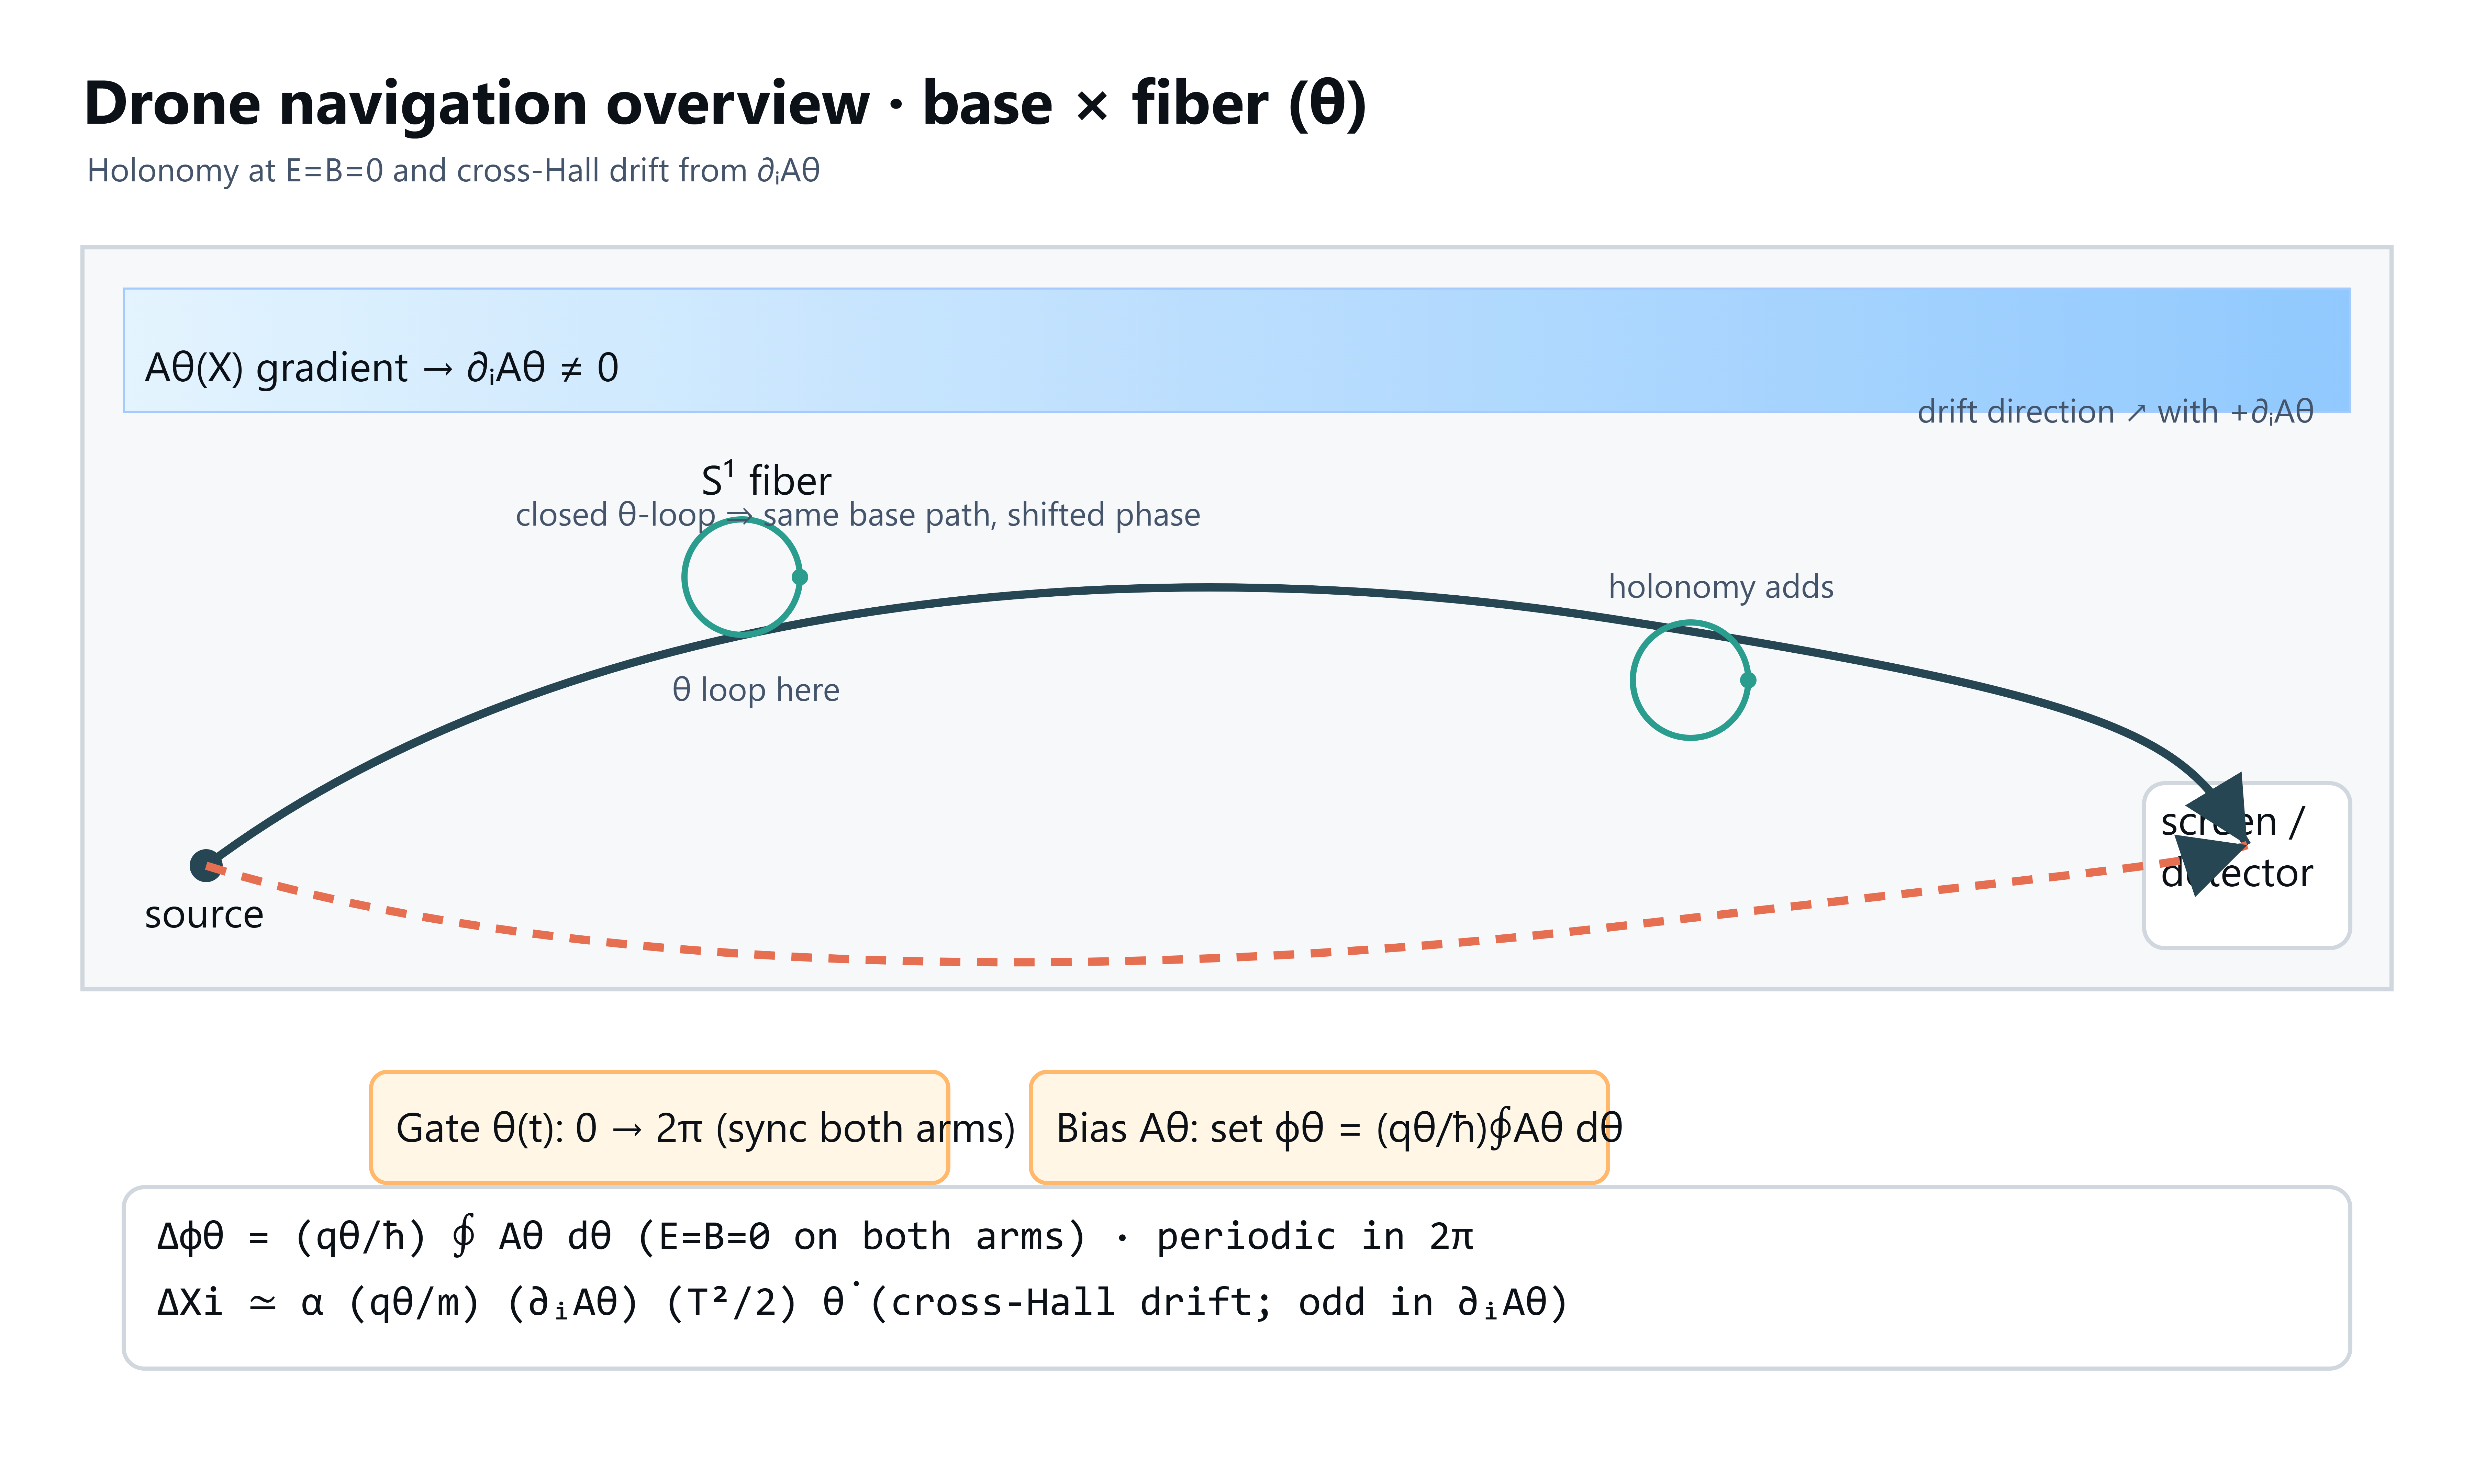
\includegraphics[width=0.75\linewidth]{drone_nav_overview.png}
	\caption{Drone navigation analogy: base motion (drone) with an internal $\theta$ dial (orange). Closing a loop on the dial leaves a holonomy $\hol$ visible at $E=B=0$ along both arms; blue arrows illustrate cross-Hall drifts when $\partial_\mu A_\theta\neq 0$.\label{fig:drone-analogy}}
\end{figure}

Pointers: lab holonomy (\cref{sec:theta-ab}), sidebands as an inertia gauge (\cref{sec:sidebands}), unified range (\cref{sec:unified-force}), and bounce/WDW barrier (\cref{sec:cosmology}).

\section{The X--\texorpdfstring{$\theta$}{theta} Mathematical Framework (Central Formalism)}\label{sec:framework}

I collect the full formalism here; later sections specialize to experiments and cosmology. To match prior drafts that used $F_{ab}$, I write the field strength on $Q$ as $G_{ab}\equiv\partial_aA_b-\partial_bA_a$ (synonymous with $F_{ab}$ earlier).

\paragraph{Units and conventions.} Unless stated otherwise, I use SI units in this section and keep $\hbar$ explicit in quantum contexts. In the relativistic St\"uckelberg completion (\cref{sec:unified-force}) I adopt natural units with $\hbar=c=1$; when needed, $\hbar$ and $c$ can be restored by dimensional analysis.

\subsection{Configuration space, connection, and curvature}\label{sec:config-connection-curvature}
\begin{align}
Q&=\mathbb{R}^{3,1}\times S^1, & q^a&=(X^\mu,\theta), & a&\in\{0,1,2,3,\theta\},\\
A&=A_a\,dq^a= A_\mu\,dX^\mu + A_\theta\,d\theta, & G&=dA, & G_{ab}&=\partial_aA_b-\partial_bA_a.
\end{align}
Key mixed component: $G_{\mu\theta}=\partial_\mu A_\theta-\partial_\theta A_\mu$.

\begin{idea}
Think of ordinary space as a city map, and add a tiny circular \emph{dial} $\theta$ at every point. Turning the dial moves you along the fiber circle without moving on the map. The connection $A$ tells you how “phase” changes as you move—on the map and around the dial. The curvature $G=dA$ measures how those changes \emph{fail to cancel} around a loop (that failure is the holonomy). A picture of this "map\,$\times$\,dial" view is shown in Fig.~\ref{fig:map-dial}.
\end{idea}

\begin{figure}[htbp]
  \centering
  \includegraphics[width=\linewidth]{UG_S2_config_space_with_theta.png}
  \caption{Configuration space as “map $\times$ dial”: every base point carries a circular fiber $\theta$. Mixed curvature $G_{\mu\theta}$ links base motion to the fiber dial.}
  \label{fig:map-dial}
\end{figure}

\paragraph{Intuition and analogies.}
\begin{itemize}
  \item \textbf{Compact dimension ($S^1$).} $Q=\mathbb R^{3,1}\times S^1$ means I add one extra circular coordinate $\theta$ (angle, period $2\pi$) to ordinary space--time. Analogy: a garden hose looks 1D from afar but has a circular cross-section up close.
  \item \textbf{Gauge connection ($A$).} A geometric bookkeeping tool for how phases change when you move: a 1-form $A=A_a dq^a=A_\mu dX^\mu + A_\theta d\theta$. Analogy: a boat's navigation aid compensating for currents so transport is consistent.
  \item \textbf{Curvature ($G=dA$) and holonomy.} Curvature measures the failure of phase changes to cancel on a loop; holonomy is the loop-induced phase. Analogy: hike a loop around a hill and your compass heading can twist.
  \item \textbf{Mixed curvature ($G_{\mu\theta}$).} Couples base motion and internal rotation; in the common gauge $\partial_\theta A_\mu=0$ this reduces to a spatial gradient $\partial_\mu A_\theta$ that produces the cross-Hall response. Analogy: meshed gears---motion in one drives the other.
\end{itemize}

\subsection{Non-relativistic Lagrangian, Hamiltonian, and currents}\label{sec:nr-lagrangian}
With Newtonian time $t$ and $\phi\equiv A_0$,
\begin{align}
L_{\mathrm{NR}}&=\frac{m}{2}\dot X^2+\frac{I}{2}\dot\theta^2+q_X A_i\dot X^i+q_\theta A_\theta\dot\theta - q_X\,\phi,\\
P_i&=m\dot X^i+q_X A_i,\quad p_\theta=I\dot\theta+q_\theta A_\theta.
\end{align}
Equations of motion:
\begin{align}
m\ddot X_i &= q_X\big(E_i + (\dot{\bm X}\times\bm B)_i\big) + q_\theta\,G_{i\theta}\,\dot\theta,\\
I\ddot\theta &= q_\theta\,G_{\theta 0}+ q_\theta\,G_{\theta i}\,\dot X^i,
\end{align}
with $E_i=-\partial_tA_i-\partial_i\phi$ and $\bm B=\nabla\times\bm A$. Quantum dynamics on $Q$:
\begin{equation}
 i\hbar\,\partial_t\psi = \left[\frac{1}{2m}(-i\hbar\nabla_X-q_X\bm A)^2 + \frac{1}{2I}(-i\hbar\partial_\theta-q_\theta A_\theta)^2 + q_X\,\phi\right]\psi.
\end{equation}
Continuity on $Q$:
\begin{align}
 \partial_t\rho + \nabla_X\!\cdot\bm J_X + \partial_\theta J_\theta&=0,\\
 \bm J_X&=\frac{1}{m}\,\mathrm{Re}[\psi^\dagger(-i\hbar\nabla_X-q_X\bm A)\psi],\quad J_\theta=\frac{1}{I}\,\mathrm{Re}[\psi^\dagger(-i\hbar\partial_\theta-q_\theta A_\theta)\psi].
\end{align}

\begin{idea}
A Lagrangian is a \emph{trip budget}: kinetic terms are fuel costs (base and $\theta$ motion), potentials are hills, and the gauge potentials $(A_i,A_\theta)$ act like tolls that depend on where and how you move. The Hamiltonian is the accountant: it doesn’t let energy vanish, it just allows it to move between base motion, fiber motion, and interactions. A single units reminder keeps this honest: $[A_\theta]=\hbar/q_\theta$, so $q_\theta A_\theta$ carries momentum units along~$\theta$.
\end{idea}

\paragraph{Units sanity (quick check).}
\begin{itemize}
  \item $[A_\theta]=\hbar/q_\theta$ so that $q_\theta A_\theta$ carries momentum units along $\theta$; $[\partial_i A_\theta]= (\hbar/q_\theta)/\text{length}$.
  \item The Lagrangian piece $q_\theta A_\theta\,\dot\theta$ has energy units; the cross-Hall force term $q_\theta (\partial_i A_\theta)\,\dot\theta$ has force units.
\end{itemize}

\paragraph{Reading the Hamiltonian (at a glance).}
\begin{itemize}
  \item Minimal coupling: $\bm p\to \bm p - q_X\bm A$ and $p_\theta\to p_\theta - q_\theta A_\theta$ incorporate forces via potentials.
  \item Two kinetic energies describe base and fiber motion: $\tfrac{1}{2m}(\cdots)^2$ and $\tfrac{1}{2I}(\cdots)^2$. The parameter $I$ is an internal moment of inertia.
  \item Continuity on $Q$ is just probability conservation on the enlarged space.
\end{itemize}

\paragraph{EP hygiene (assumption).} To avoid composition-dependent violations of the equivalence principle at leading order, I take the $\theta$-charge to be composition-independent (e.g., $Q_\theta=\beta m$ or $\propto B\! -\!L$). This makes the new force universal at first approximation and is consistent with E\"otv\"os-type constraints; any residual composition dependence then only arises via the tiny portal mixings in \cref{sec:unified-force}.

Rotor spectrum and holonomy shift:
\begin{equation}
 E_\ell=\frac{\hbar^2}{2I}\Big(\ell-\frac{\phi_\theta}{2\pi}\Big)^2,\qquad \phi_\theta\equiv\frac{q_\theta}{\hbar}\oint A_\theta\,d\theta,\qquad \ell\in\mathbb Z.
\end{equation}

\subsection{Relativistic worldline, massless limit, and covariant wave equation}\label{sec:relativistic-worldline}
Worldline action with einbein $e(\tau)$ and metric $G^{(\mathrm{geom})}_{ab}dq^adq^b=\eta_{\mu\nu}dX^\mu dX^\nu+\kappa^2 d\theta^2$:
\begin{equation}
 S_{\mathrm{rel}}=\int d\tau\Big[\frac{1}{2e}\,G^{(\mathrm{geom})}_{ab}\,\dot q^a\dot q^b - \frac{e}{2}\,m^2 + q_X A_\mu\dot X^\mu + q_\theta A_\theta\dot\theta\Big].
\end{equation}

    \begin{idea}
      	\textbf{Worldline, in one picture.} Imagine a tram on a flexible track that sags where heavy objects sit. The tram \emph{must} follow those curves. A particle’s worldline is the tram’s path; mass and curvature bend spacetime the way weights bend the track. Tracing the worldline is simply tracing that path through time.
    \end{idea}
Mass-shell constraint $G^{ab}_{\mathrm{(geom)}}(P_a-q_aA_a)(P_b-q_bA_b)+m^2=0$. In the NR limit $I=m\kappa^2$.

\paragraph{Worldline and einbein (at a glance).}
\begin{itemize}
  \item The path is parametrized by $\tau$; the einbein $e(\tau)$ keeps the action reparametrization-invariant.
  \item Varying $e$ enforces the mass-shell condition that reduces to $E^2=\bm p^2+m^2$ when fields vanish.
  \item The added metric piece $\kappa^2 d\theta^2$ says motion in $\theta$ contributes to the worldline length; in the NR limit one finds $I=m\kappa^2$.
  \item Intuition: the einbein is like a choice of speedometer; it sets the clock along the path without changing the trip.
\end{itemize}

Covariant wave equation on $Q$ (scalar):
\begin{equation}
 \big[D_\mu D^\mu + \kappa^{-2} D_\theta^2 + m^2\big]\,\Psi(X,\theta)=0,\quad D_\mu=\partial_\mu+\tfrac{i}{\hbar}q_XA_\mu,\; D_\theta=\partial_\theta+\tfrac{i}{\hbar}q_\theta A_\theta.
\end{equation}

  \begin{idea}
  	  	\textbf{Covariant waves.} Think of raindrop ripples on a pond. From the shore or from a raft, the pattern \emph{looks} different, but the water’s rule is the same. The covariant wave equation is that universal rule: one description that stays consistent in any coordinates while the ripple can also wrap around the compact $\theta$ direction.
  \end{idea}

\paragraph{Massless limit (\texorpdfstring{$m\to 0$}{m->0}).} With finite $\kappa_0$,
\begin{equation}
 S_{m=0}=\int d\tau\Big[\frac{1}{2e}(\eta_{\mu\nu}\dot X^\mu\dot X^\nu+\kappa_0^2\dot\theta^2)+q_X A_\mu\dot X^\mu+q_\theta A_\theta\dot\theta\Big],\quad \eta_{\mu\nu}\dot X^\mu\dot X^\nu+\kappa_0^2\dot\theta^2=0.
\end{equation}

\paragraph{NR map.} Removing the rest-energy phase yields the Schr\"odinger equation in \cref{sec:nr-lagrangian} provided I identify $\boxed{\ I=m\kappa^2\ }$.

\begin{idea}
Two pictures: the \emph{rubber sheet} (curvature makes dimples that steer motion) and the \emph{ripple} (the covariant wave equation moves ripples consistently in any good coordinates). The fiber just adds one compact direction the ripple can wrap around; the NR limit packages it into the rotor inertia $I=m\kappa^2$.
\end{idea}

\paragraph{Parameter map.} The rotor inertia $I$ is a probe property tied to geometry via $I=m\kappa^2$, whereas the 4D vector mass $m_\theta=g_\theta f_\theta$ in the St\"uckelberg completion is a mediator property controlling the shared Yukawa range $\lambda_\theta=1/m_\theta$ (\cref{sec:unified-force}).

\subsection{Gauge invariance on \texorpdfstring{$Q$}{Q} and large loops}\label{sec:gauge-invariance}
Gauge transformations: $A_\mu\to A_\mu+\partial_\mu\Lambda_X$, $A_\theta\to A_\theta+\partial_\theta\Lambda_\theta$, with $\psi\to \exp\!\left[-\tfrac{i}{\hbar}(q_X\Lambda_X+q_\theta\Lambda_\theta)\right]\psi$. Under a large gauge transformation around the circle, $\oint A_\theta d\theta \to \oint A_\theta d\theta + 2\pi\,\hbar/q_\theta$, so only $\phi_\theta$ modulo $2\pi$ is physical.

\begin{idea}
Changing gauge is like moving the zero mark on an altimeter: the mountain stays the same. Only \emph{closed loops} reveal structure. March once around the fiber circle and you collect a net phase $\phi_\theta=\tfrac{q_\theta}{\hbar}\oint A_\theta d\theta$, but physics cares only modulo $2\pi$ (large–gauge periodicity).
\end{idea}

\begin{figure}[htbp]
  \centering
  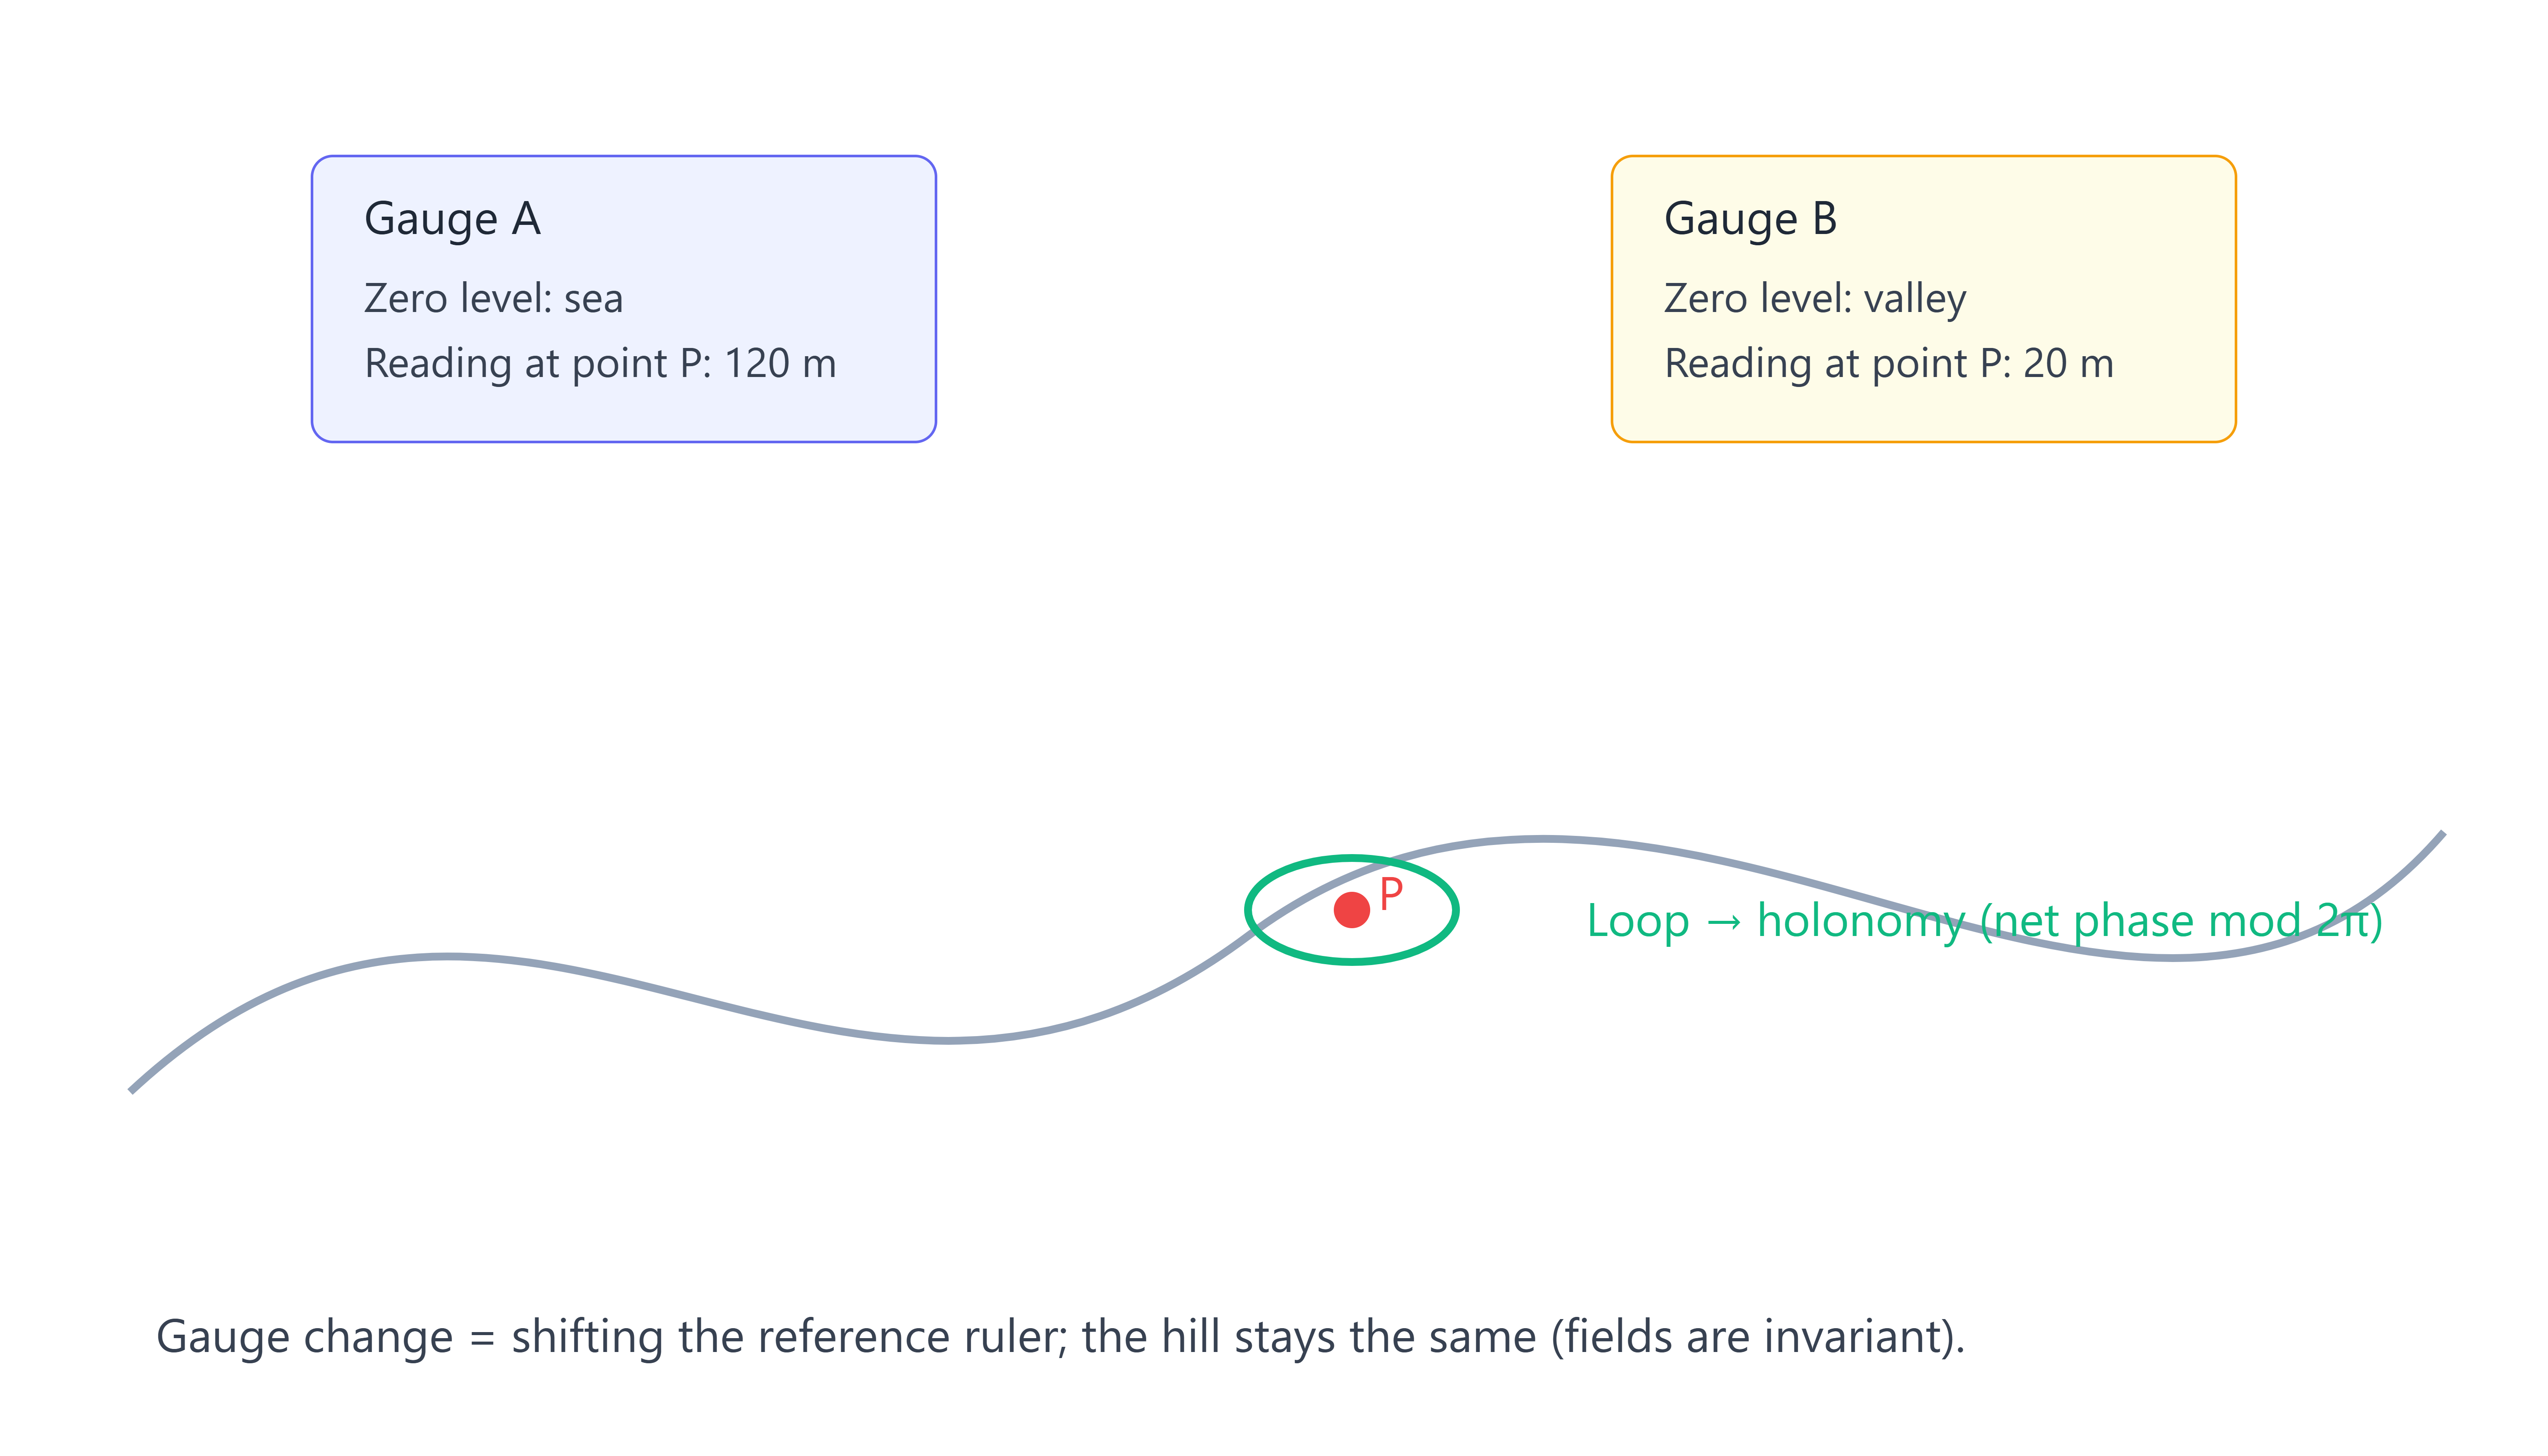
\includegraphics[width=\linewidth]{UG_S2_gauge_and_holonomy.png}
  \caption{Gauge change shifts the reference, not the hill. A closed loop probes holonomy; only $\phi_\theta\ (\bmod\ 2\pi)$ is observable.}
  \label{fig:ug-holonomy}
\end{figure}

The Bianchi identity $dG=0$ holds for $G=dA$ when one treats $(A_\mu, A_\theta)$ as components of a single connection; in many experiments I choose $\partial_\theta A_\mu=0$, leaving the measurable gradient $\partial_\mu A_\theta$.

\begin{figure}[htbp]
  \centering
  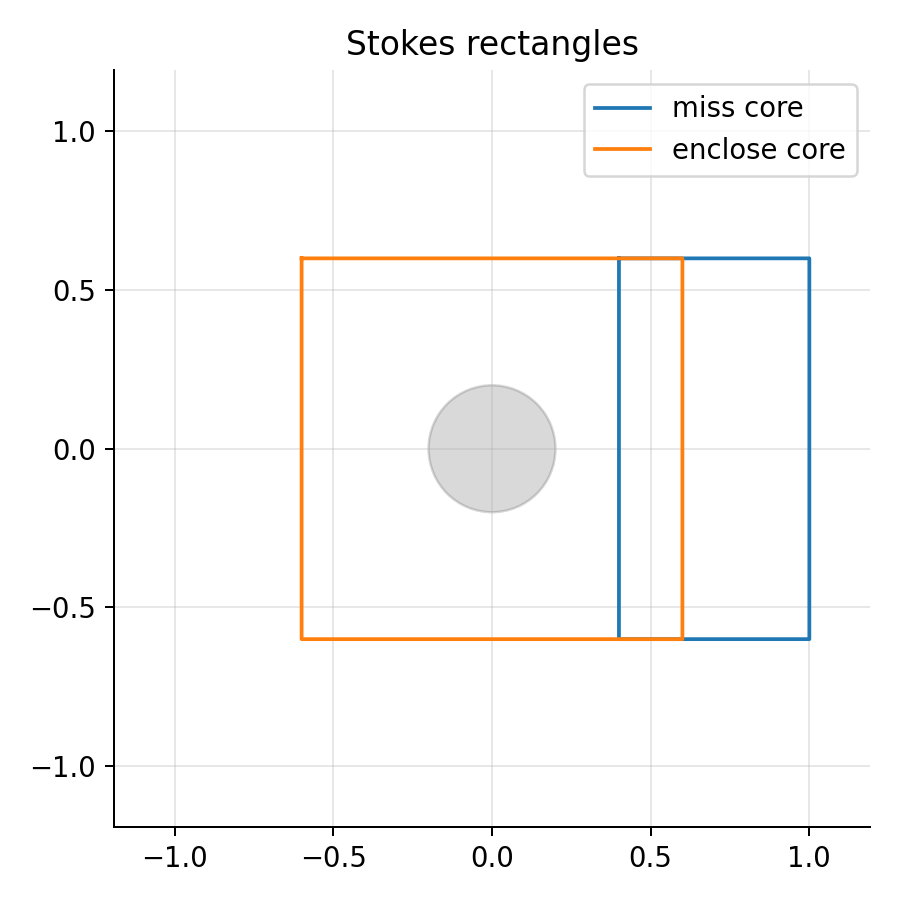
\includegraphics[width=0.6\linewidth]{stokes_rectangles.png}
  \caption{Holonomy schematic: Stokes rectangles visualize how loop integrals relate to enclosed curvature; only the loop integral modulo the large-gauge period is observable.}
  \label{fig:stokes}
\end{figure}

\subsection{Consistency checks \& known limits}\label{sec:consistency-checks}
\begin{itemize}
  \item \textbf{Turning off the fiber ($I\to\infty$, $q_\theta\to 0$).} Dynamics reduce to standard electrodynamics and quantum mechanics on $\mathbb R^{3,1}$: no $A_\theta$ phases and no rotor sidebands.
  \item \textbf{Turning off base electromagnetism ($q_X\to 0$).} The system is a free internal rotor that can still depend on $X$ through $A_\theta(X)$; sidebands with spacing $\Delta E\approx \hbar^2/(2I)$ and the $\theta$--AB phase $\Delta\phi_\theta=\tfrac{q_\theta}{\hbar}\oint A_\theta d\theta$ persist.
  \item \textbf{Relativistic $\to$ non-relativistic.} Identifying $I=m\kappa^2$ ensures the Schr\"odinger equation inherits the correct rotor term $\tfrac{1}{2I}(-i\hbar\partial_\theta-q_\theta A_\theta)^2$ after removing the rest-energy phase.
\end{itemize}

\subsection{Worked reductions (one screen)}\label{sec:worked-reductions}
I summarize the $I\to\infty$, $q_X\to 0$, and $I=m\kappa^2$ limits and their outcomes for observables (sidebands, holonomy) and consistency.

\section{Phenomena \& Tests (Lab and Null-EM Signatures)}\label{sec:phenomenology}

Convention: “Fiber-off” means $I\to\infty$ and $q_\theta\to 0$.

\subsection{\texorpdfstring{$\theta$}{theta}--AB phase under null spatial fields}\label{sec:theta-ab}
Action contribution along a closed internal loop $\mathcal C_\theta$ yields a path-integral phase $\exp[i(q_\theta/\hbar)\oint A_\theta d\theta]$. The observable phase is
\begin{equation}
 \Delta\phi_\theta = \frac{q_\theta}{\hbar}\oint A_\theta\,d\theta \pmod{2\pi},\qquad \bm E=\bm B=0.
\end{equation}

\begin{idea}
Like a note sounding different in two rooms, the \emph{phase} can shift even when $\mathbf{E}=\mathbf{B}=0$ along both arms. Here the hidden dial $\theta$ supplies the shift: $\Delta\phi_\theta=\phi_\theta$ (\(\bmod\ 2\pi\)), so sweeping $\phi_\theta$ by $2\pi$ brings the fringes right back.
\end{idea}

\begin{figure}[htbp]
  \centering
  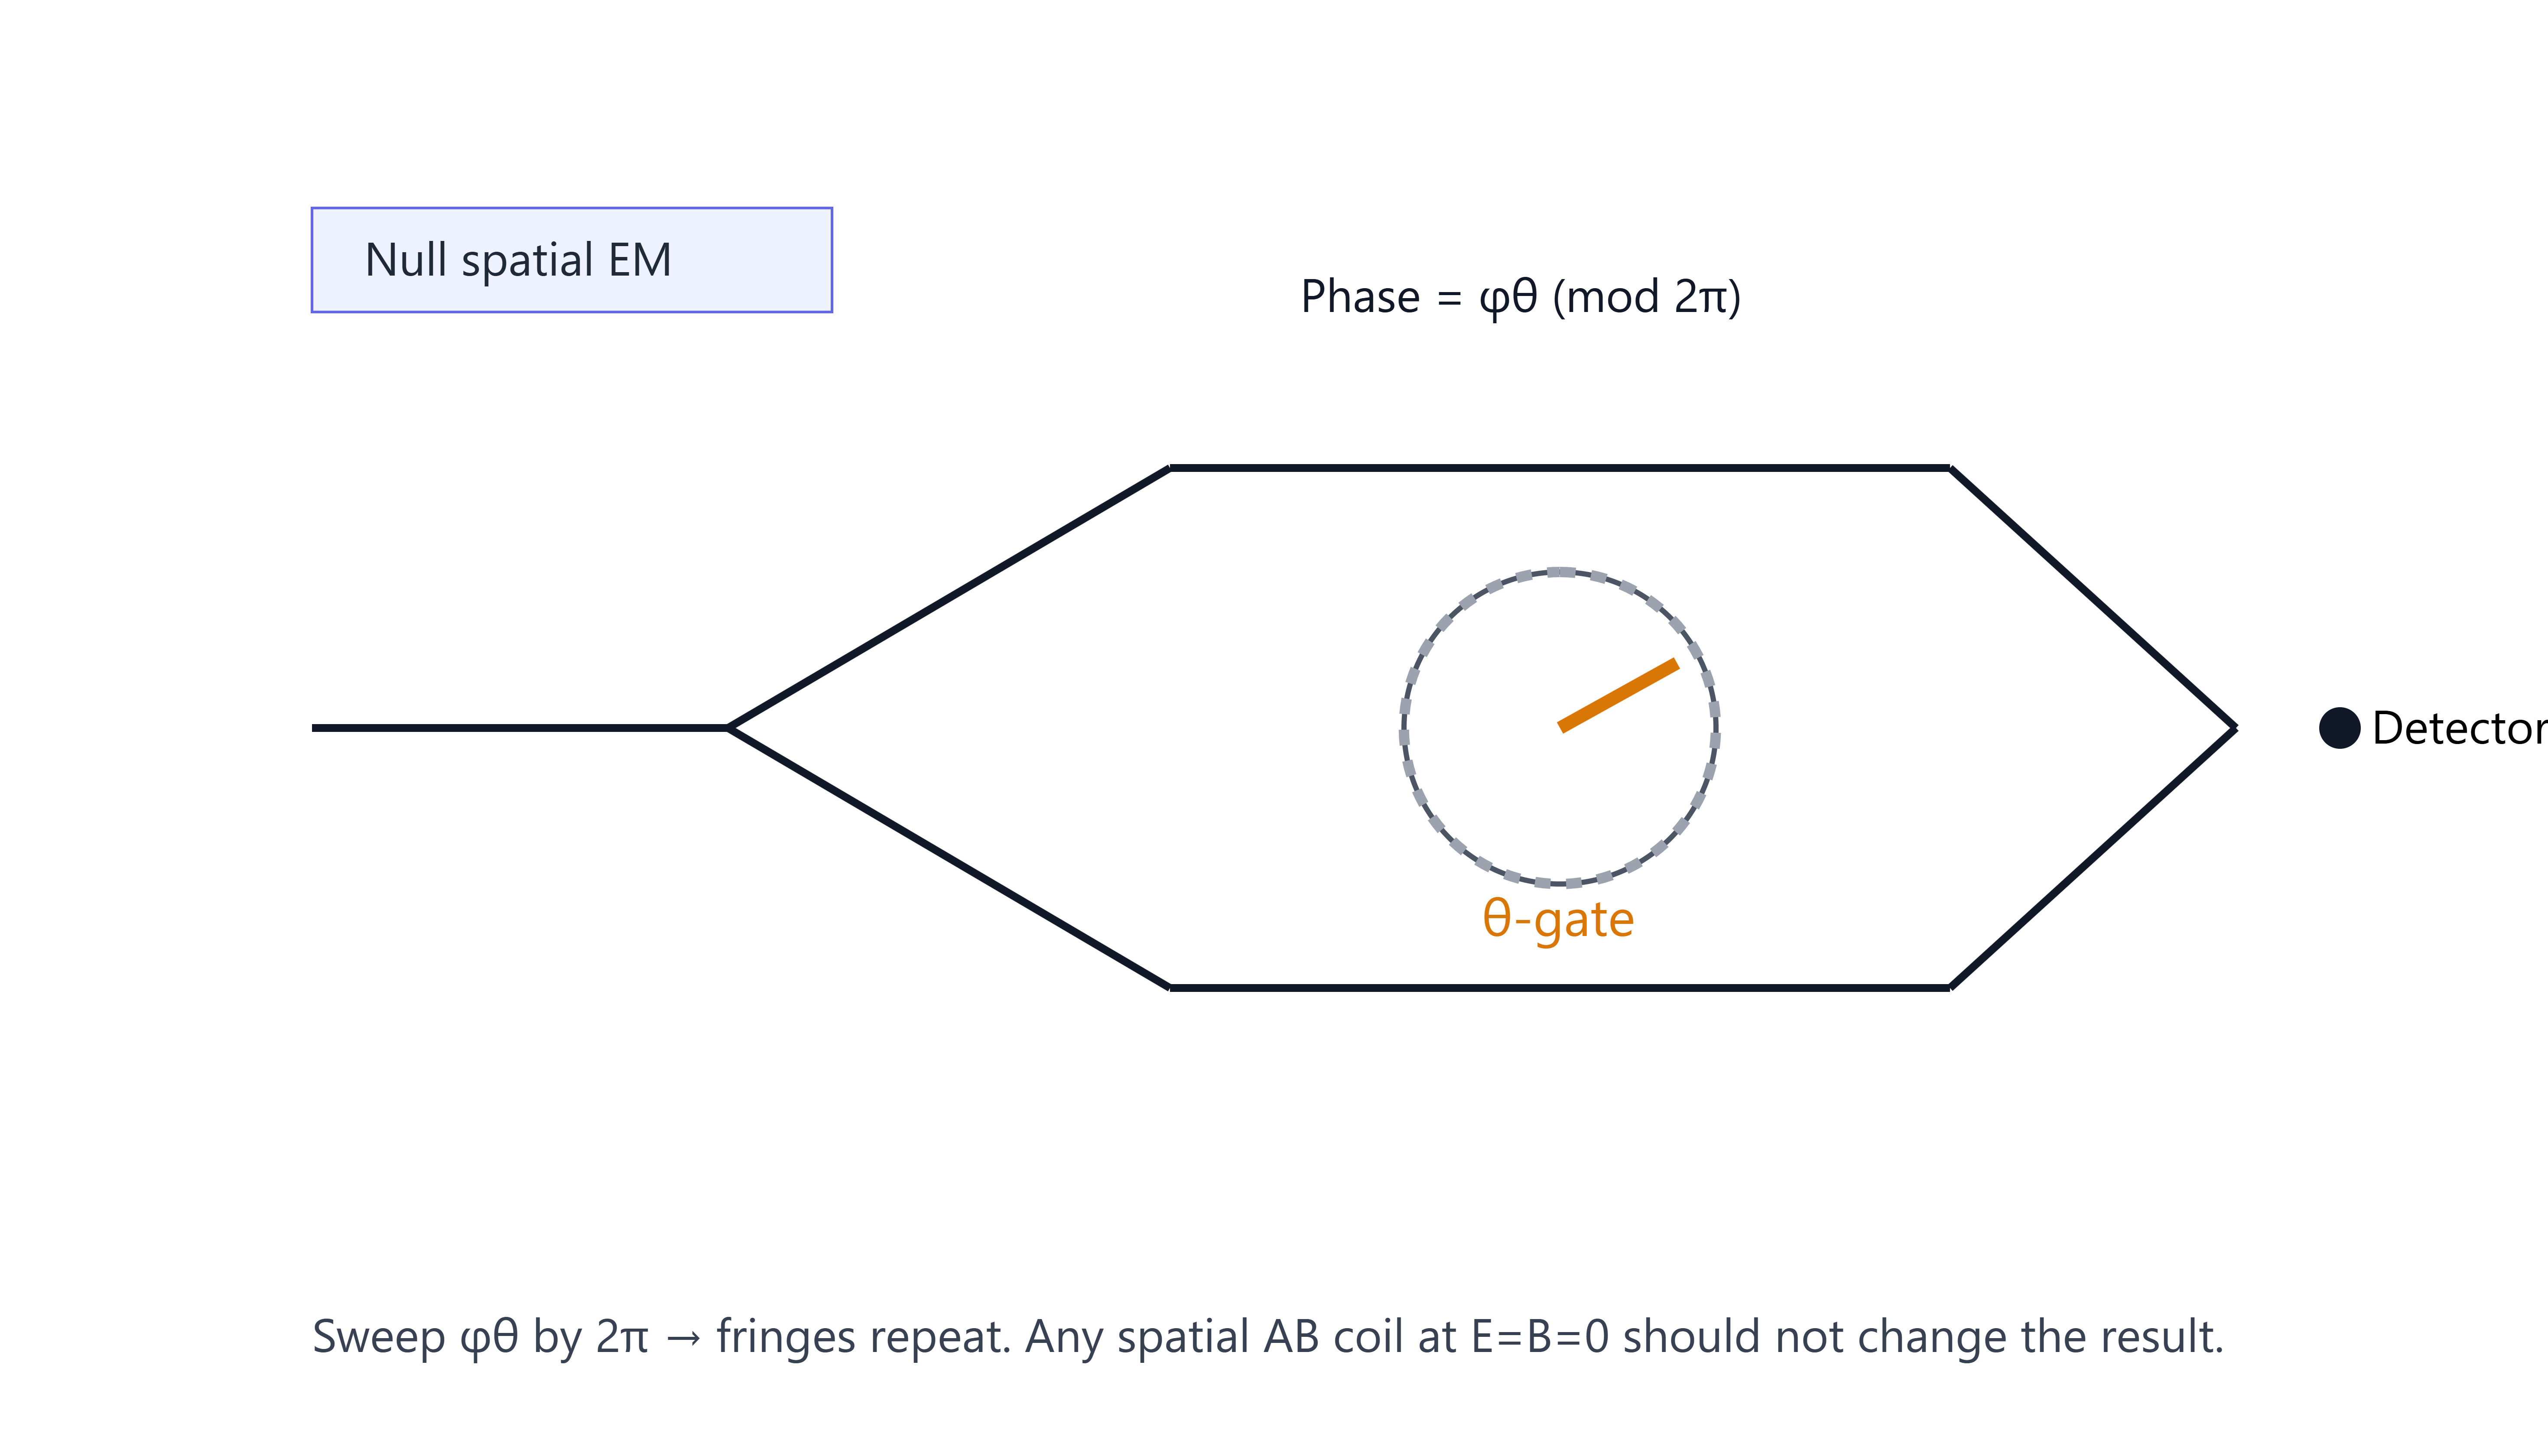
\includegraphics[width=\linewidth]{UG_S3_theta_AB.png}
  \caption{$\theta$--AB interferometer at null spatial EM. The $\theta$-gate dials $\phi_\theta$; fringes are strictly $2\pi$-periodic.}
  \label{fig:theta-ab-cartoon}
\end{figure}

\begin{figure}[htbp]
  \centering
  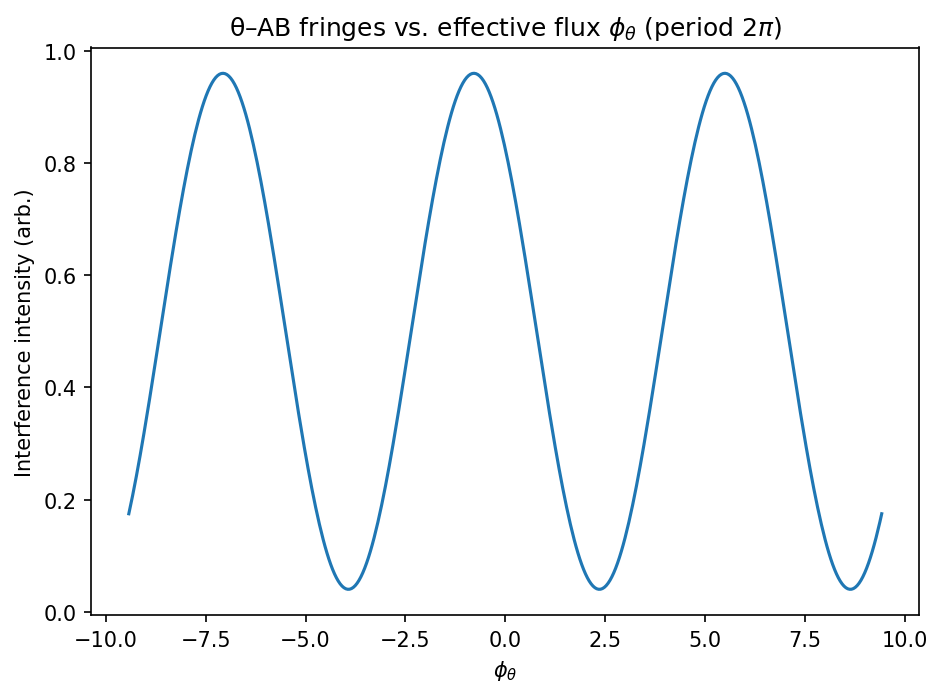
\includegraphics[width=0.7\linewidth]{exp1_fringe_vs_phi.png}
  \caption{Fringe vs. $\phi_\theta$ (simulation).}
  \label{fig:theta-ab-fringe}
\end{figure}

\csvnote{../paper/data/exp1_theta_ab_fringe.csv}

\subsection{Cross-Hall drift from mixed curvature}\label{sec:cross-hall}
With $\bm E=\bm B=0$, $m\ddot X_i = q_\theta\,G_{i\theta}\,\dot\theta$ ($G_{i\theta}=\partial_iA_\theta-\partial_\theta A_i$). For a uniform gate of duration $T$ and nearly constant $\dot\theta$,
\begin{equation}
 \Delta X_i \simeq \alpha\,\frac{q_\theta}{m}\,(\partial_iA_\theta)\,\frac{T^2}{2}\,\dot\theta,\qquad \alpha\lesssim 1.
\end{equation}

\begin{idea}
A hidden current can push a boat sideways. Likewise a gradient $\partial_y A_\theta$ plus a time window with $\dot\theta\neq 0$ nudges the packet: $\Delta y\propto(\partial_y A_\theta)\,\dot\theta\,T^2$. Flip either sign and the drift reverses; turn either off and it vanishes.
\end{idea}

\begin{figure}[htbp]
  \centering
  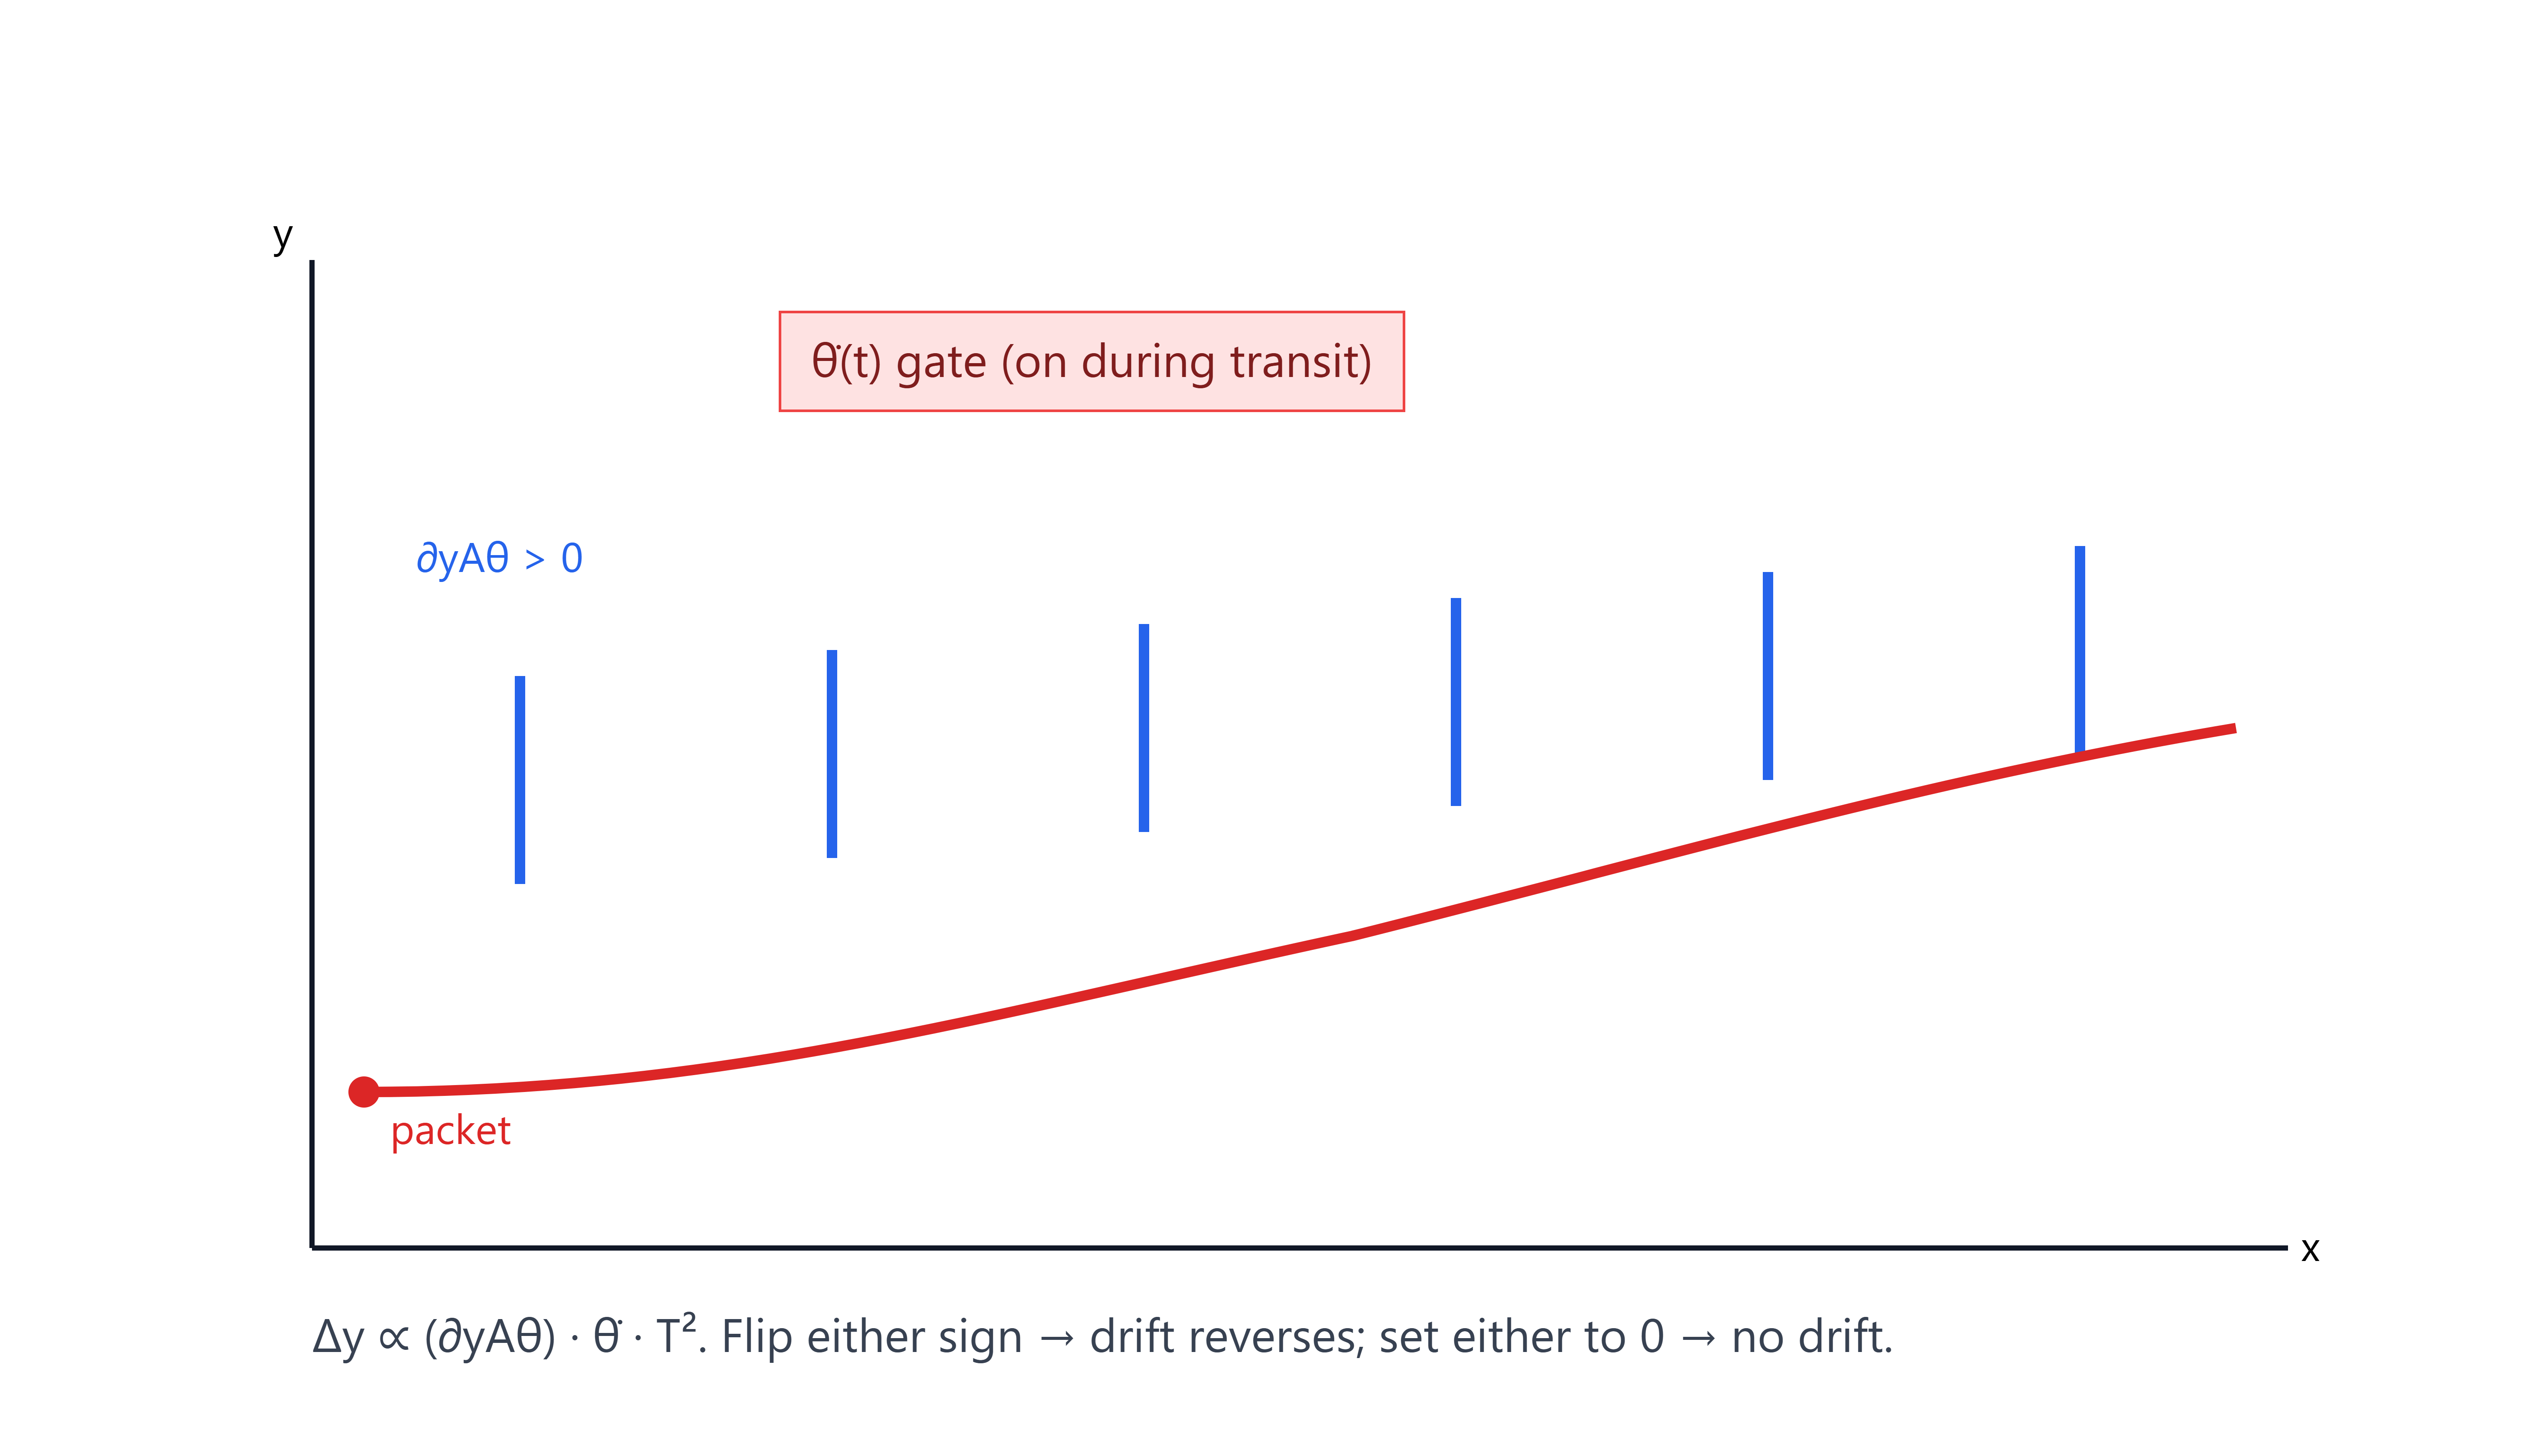
\includegraphics[width=\linewidth]{UG_S3_cross_hall.png}
  \caption{Cross\textendash Hall drift intuition: blue arrows for $\partial_yA_\theta$, red packet deflection.}
  \label{fig:cross-hall-cartoon2}
\end{figure}

\begin{figure}[htbp]
  \centering
  \begin{subfigure}[b]{0.48\linewidth}
    \centering
    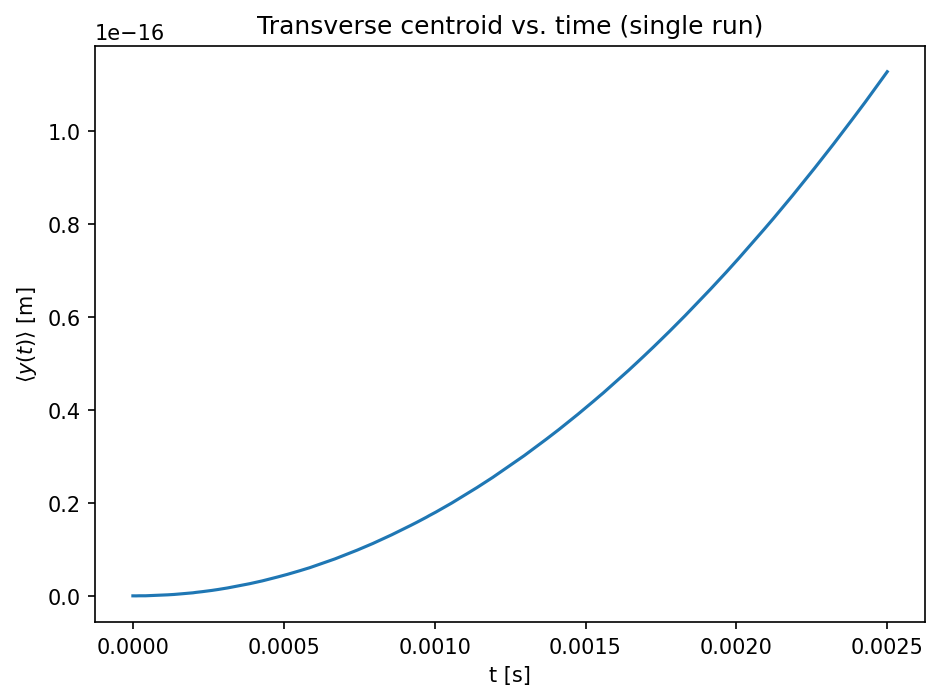
\includegraphics[width=\linewidth]{exp2_y_traj.png}
    \caption{Centroid trajectory $\langle y(t)\rangle$}
    \label{fig:cross-hall-traj}
  \end{subfigure}\hfill
  \begin{subfigure}[b]{0.48\linewidth}
    \centering
    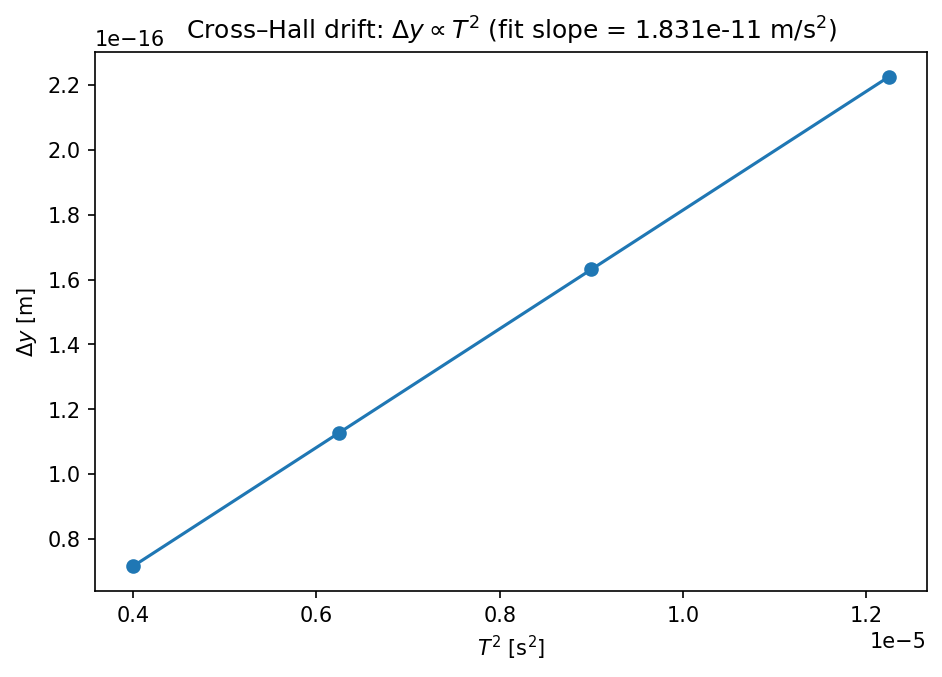
\includegraphics[width=\linewidth]{exp2_dy_vs_T2.png}
    \caption{$\Delta y$ vs $T^2$ scaling}
    \label{fig:cross-hall-scaling}
  \end{subfigure}
  \caption{Cross\textendash Hall drift: simulation traces and $T^2$ scaling.}
  \label{fig:cross-hall}
\end{figure}

\csvnote{../paper/data/exp2_drift_T2.csv}

\subsection{Sidebands from the rotor Hamiltonian}\label{sec:sidebands}
Separating variables $\Psi=\sum_{\ell}\psi_\ell(X)e^{i\ell\theta}$ yields rotor levels $E_\ell=\frac{\hbar^2}{2I}(\ell-\phi_\theta/2\pi)^2$ and nearest-neighbor spacing $\Delta E\approx\hbar^2/(2I)$.

\begin{figure}[htbp]
  \centering
  \begin{subfigure}[b]{0.48\linewidth}
    \centering
  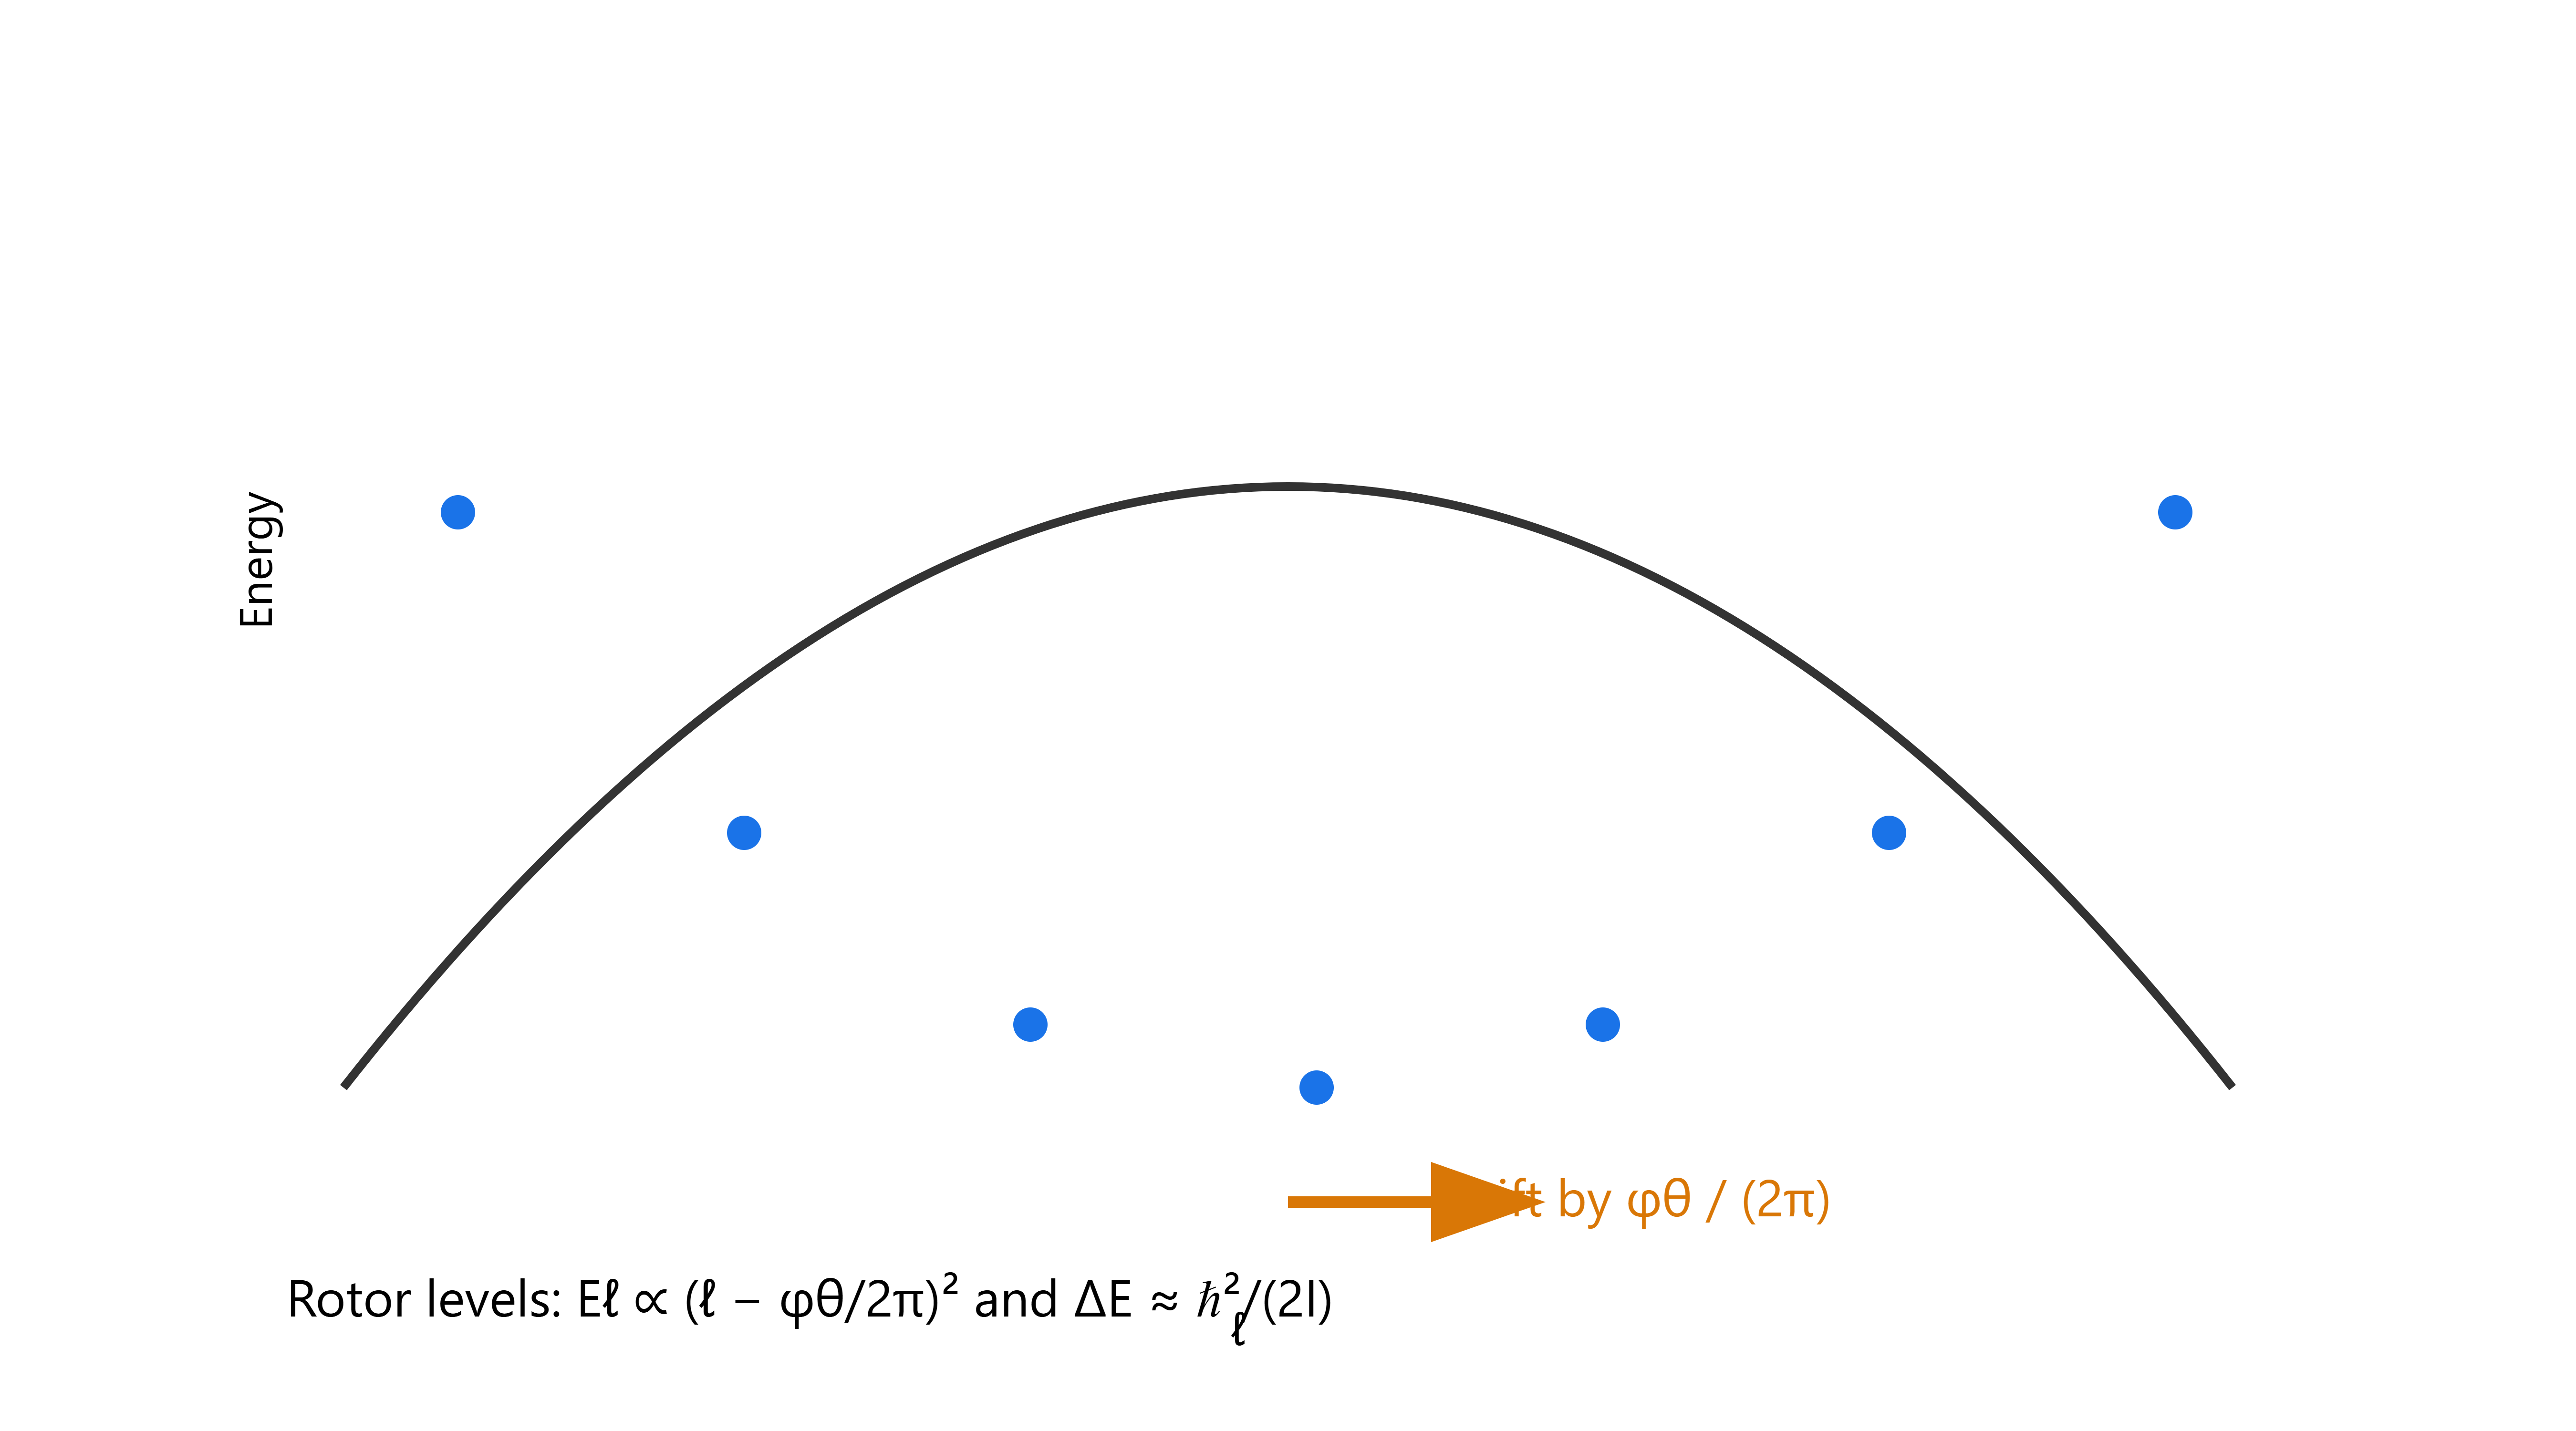
\includegraphics[width=\linewidth]{S3_rotor_levels_cartoon.png}
    \caption{Rotor levels (cartoon)}
    \label{fig:rotor-cartoon}
  \end{subfigure}\hfill
  \begin{subfigure}[b]{0.48\linewidth}
    \centering
    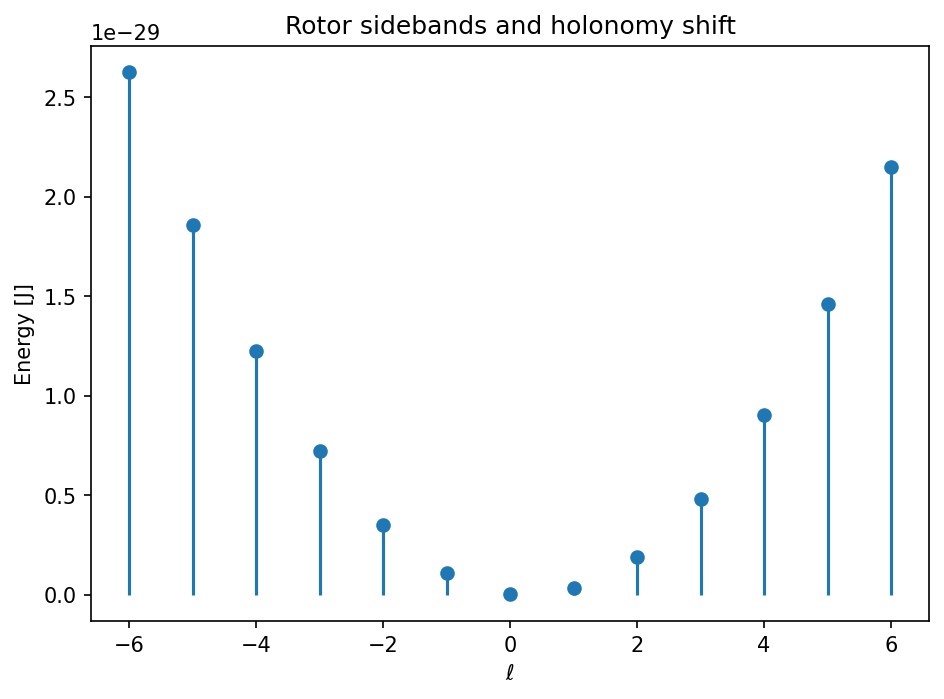
\includegraphics[width=\linewidth]{exp3_rotor_levels.png}
    \caption{Rotor levels (simulation)}
    \label{fig:rotor-sim}
  \end{subfigure}
  \begin{subfigure}[b]{0.48\linewidth}
    \centering
  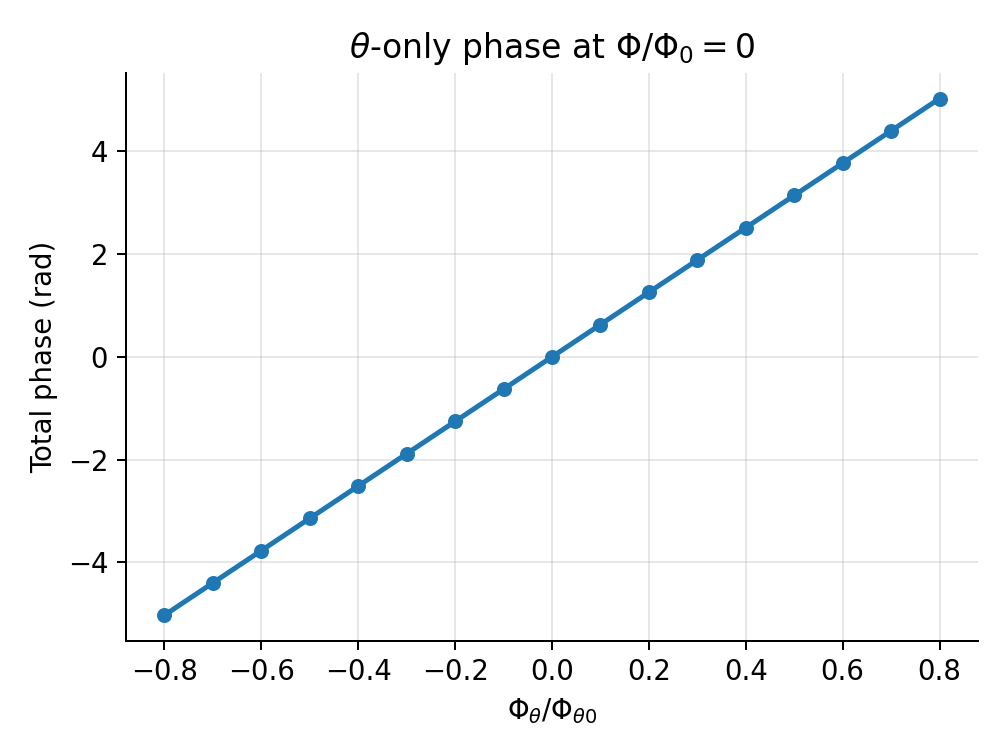
\includegraphics[width=\linewidth]{theta_only.png}
    \caption{$\theta$-only baseline}
    \label{fig:theta-only}
  \end{subfigure}
  \caption{Rotor sidebands and $\theta$-only baseline.}
  \label{fig:rotor}
\end{figure}

\csvnote{../paper/data/exp3_rotor_levels.csv}

\subsection{Order-of-magnitude anchors for \texorpdfstring{$I$}{I}}\label{sec:iom}
$\Delta E=h\,\Delta f$, $\ I\approx \hbar^2/(2\,\Delta E)$. Example: $\Delta f=\SI{1}{Hz}\Rightarrow I\approx 8.4\times 10^{-36}\,\mathrm{J\,s^2}$.

\subsection{Falsification protocol}\label{sec:falsification}
Vary spatial flux at fixed $\phi_\theta$; enforce $2\pi$ periodicity in $\phi_\theta$; use closed $\theta$-loop controls and arm swaps.

\subsection{Consistency checks \& limits (QM/NR)}\label{sec:lab-consistency}
Fiber-off ($I\to\infty$, $q_\theta\to 0$), pure $\theta$ sector ($q_X\to 0$), large-gauge periodicity in $\oint A_\theta d\theta$.

\subsection{Methods: \texorpdfstring{$\theta$}{theta}--Aharonov--Bohm interferometer}\label{sec:methods-theta-ab}
Program a $\theta(t)$ modulation that advances by $2\pi N_\theta$ during the arm transit; if $A_\theta$ is approximately constant along the path in $\theta$, then $\Delta\phi_\theta \approx (q_\theta/\hbar) A_\theta (2\pi N_\theta)$.

\begin{figure}[htbp]
  \centering
  \begin{subfigure}[b]{0.48\linewidth}
    \centering
  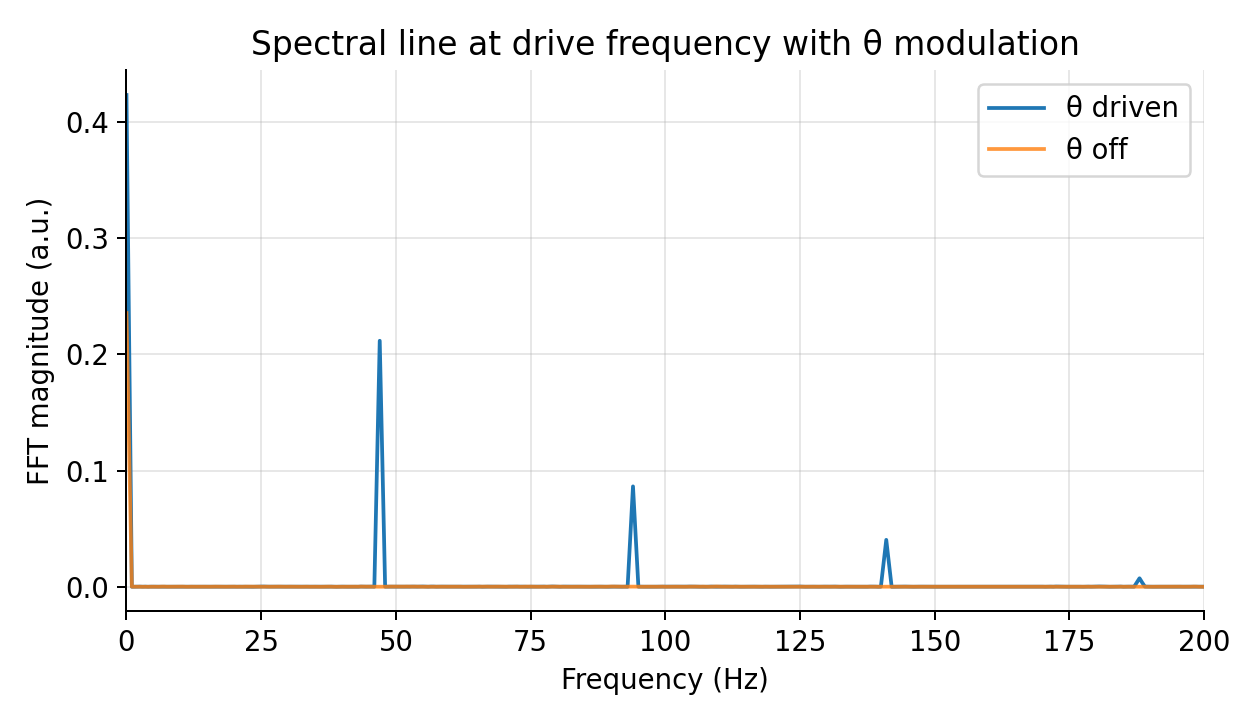
\includegraphics[width=\linewidth]{fft_theta_drive.png}
    \caption{FFT of a sample $\theta$ drive}
    \label{fig:fft-theta}
  \end{subfigure}\hfill
  \begin{subfigure}[b]{0.48\linewidth}
    \centering
  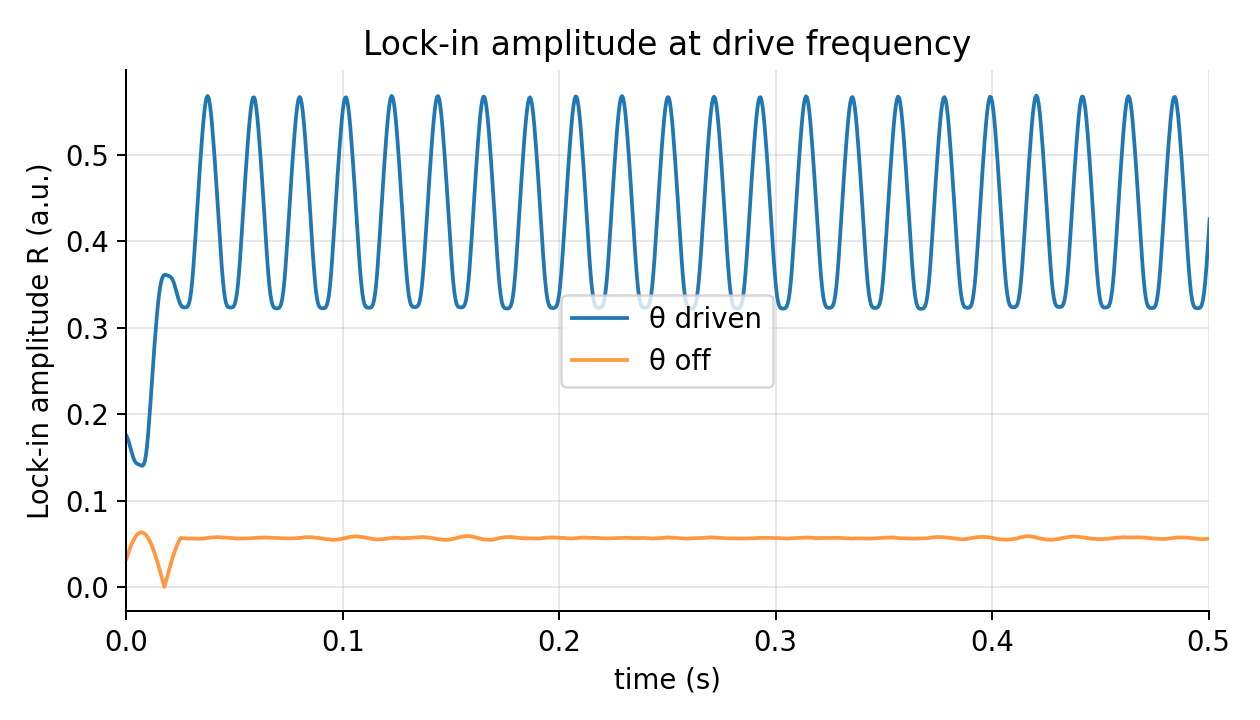
\includegraphics[width=\linewidth]{lockin_theta_drive.png}
    \caption{Lock-in demodulation concept}
    \label{fig:lockin-theta}
  \end{subfigure}
  \caption{Method visuals for $\theta$--AB interferometry.}
  \label{fig:methods}
\end{figure}

\subsection{Mesoscopic Transport: AB Rings with a \texorpdfstring{$\theta$}{theta}-Flux Offset}\label{sec:mesoscopic}
$G(\Phi,\Phi_\theta)\propto \cos[2\pi(\Phi/\Phi_0+\Phi_\theta/\Phi_{\theta,0})]$, $\Phi_{\theta,0}=2\pi\hbar/q_\theta$.

\subsection{Singularity seam: where classical GR fails and QM fixes}\label{sec:singularity-seam}
Classical FRW: stiff $a^{-6}$ alone doesn’t bounce; adding curvature ($-k/a^2$ with $k>0$) creates a turning point. Wheeler--DeWitt adds a repulsive $+C/a^2$ barrier that blocks $a\to 0$.

\section*{Experimental Details, SNR, and Error Budgets}

\subsection*{Interferometric phase @ null spatial EM (\texorpdfstring{$\theta$--AB}{theta--AB})}
\textbf{Signal model.} $I(\phi_\theta)=\tfrac{1}{2}\!\left[1+V\cos(\phi_\theta+\phi_0)\right]$ with visibility $V\in[0,1]$.
For $N$ detected quanta per point, the shot-noise limited phase uncertainty is
$\sigma_\phi \approx 1/\sqrt{N V^2}$ (small-angle, high-contrast). I sweep $\phi_\theta\in[-4\pi,4\pi]$.

\textbf{Falsification gate.} A $2\pi$-periodic fit must achieve reduced $\chi^2\!\lesssim\!1.5$ and circular-variance of residuals $<0.1\,\mathrm{rad}^2$; dependence on any spatial AB toggle at $E{=}B{=}0$ must be $<2\sigma$ of shot noise.
\csvnote{../paper/data/exp1_theta_ab_fringe.csv}

\subsection*{Cross\textendash Hall drift}
\textbf{Signal model.} $\Delta y = \alpha\,(\partial_y A_\theta)\,\dot\theta\,T^2$. Reverse either $\partial_y A_\theta$ or $\dot\theta$ $\Rightarrow$ $\Delta y\!\to\! -\Delta y$.

\textbf{Uncertainty.} Centroid error $\sigma_y \simeq w/\sqrt{N}$ (spot size $w$); slope uncertainty from linear fit of $\Delta y$ vs $T^2$.  
\textbf{Falsification gate.} $R^2(\Delta y\text{ vs }T^2)\!>\!0.95$ \emph{and} correct sign flips; otherwise reject.
\csvnote{../paper/data/exp2_drift_T2.csv}

\subsection*{Rotor sidebands}
\textbf{Signal model.} $E_\ell=\frac{\hbar^2}{2I}\big(\ell-\frac{\phi_\theta}{2\pi}\big)^2$.  
\textbf{Fit.} Quadratic fit residual RMS $<\tfrac{1}{3}$ linewidth; holonomy shift periodic in $2\pi$.  
\csvnote{../paper/data/exp3_rotor_levels.csv}

\subsection*{Bounce and shared-range tests}
$a_{\min}=\big[(A+\Sigma^2)/k\big]^{1/4}$ with $A=\tfrac{8\pi G}{3}\,\tfrac{\Pi_\theta^2}{2I_0}$.  
\csvnote{../paper/data/exp4_bounce_scan.csv}, \csvnote{../paper/data/exp5_yukawa_profiles.csv}

\section{Cosmology Link --- From Minisuperspace to a Bounce}\label{sec:cosmology}

I sketch classical and quantum pictures in a spatially flat FRW minisuperspace with scale factor $a(t)$ and homogeneous $\theta(t)$.

\subsection{Choice of \texorpdfstring{$I$}{I}: FRW (stiff) vs. WDW (barrier)}\label{sec:i-of-a}
For FRW, take $I=I_0$ (constant). Then
\begin{equation}
\rho_\theta(a) = \frac{\Pi_\theta^2}{2 I_0\,a^6},\qquad \Pi_\theta\equiv a^3\,(I_0\,\dot\theta+q_\theta A_\theta)=\text{const},\quad w=1.
\end{equation}
For WDW, separating $\Psi=\chi(a)e^{i\ell\theta}$ gives a repulsive inverse-square barrier $+\ell^2\hbar^2/(2 I_0 a^2)$.

\subsection{Classical bounce (self-balanced \texorpdfstring{$a^{-6}$}{a^-6} and effective potential)}\label{sec:classical-bounce}
Early-time Friedmann with positive shear-like piece $+\Sigma^2/a^6$ and curvature $-k/a^2$ ($k>0$):
\begin{equation}
 H^2 = \frac{8\pi G}{3}\left(\rho_{\mathrm{std}} + \frac{\Pi_\theta^2}{2 I_0\,a^6}\right) + \frac{\Sigma^2}{a^6} - \frac{k}{a^2} \, .
\end{equation}
Defining $A\equiv \tfrac{8\pi G}{3}\tfrac{\Pi_\theta^2}{2I_0}$ and neglecting $\rho_{\mathrm{std}}$ at early times,
\begin{equation}
 H^2=\frac{A+\Sigma^2}{a^6} - \frac{k}{a^2},\qquad a_{\min}=\Big(\frac{A+\Sigma^2}{k}\Big)^{\!1/4} .
\end{equation}

\begin{figure}[h]
  \centering
  \begin{subfigure}[b]{0.48\linewidth}
    \centering
  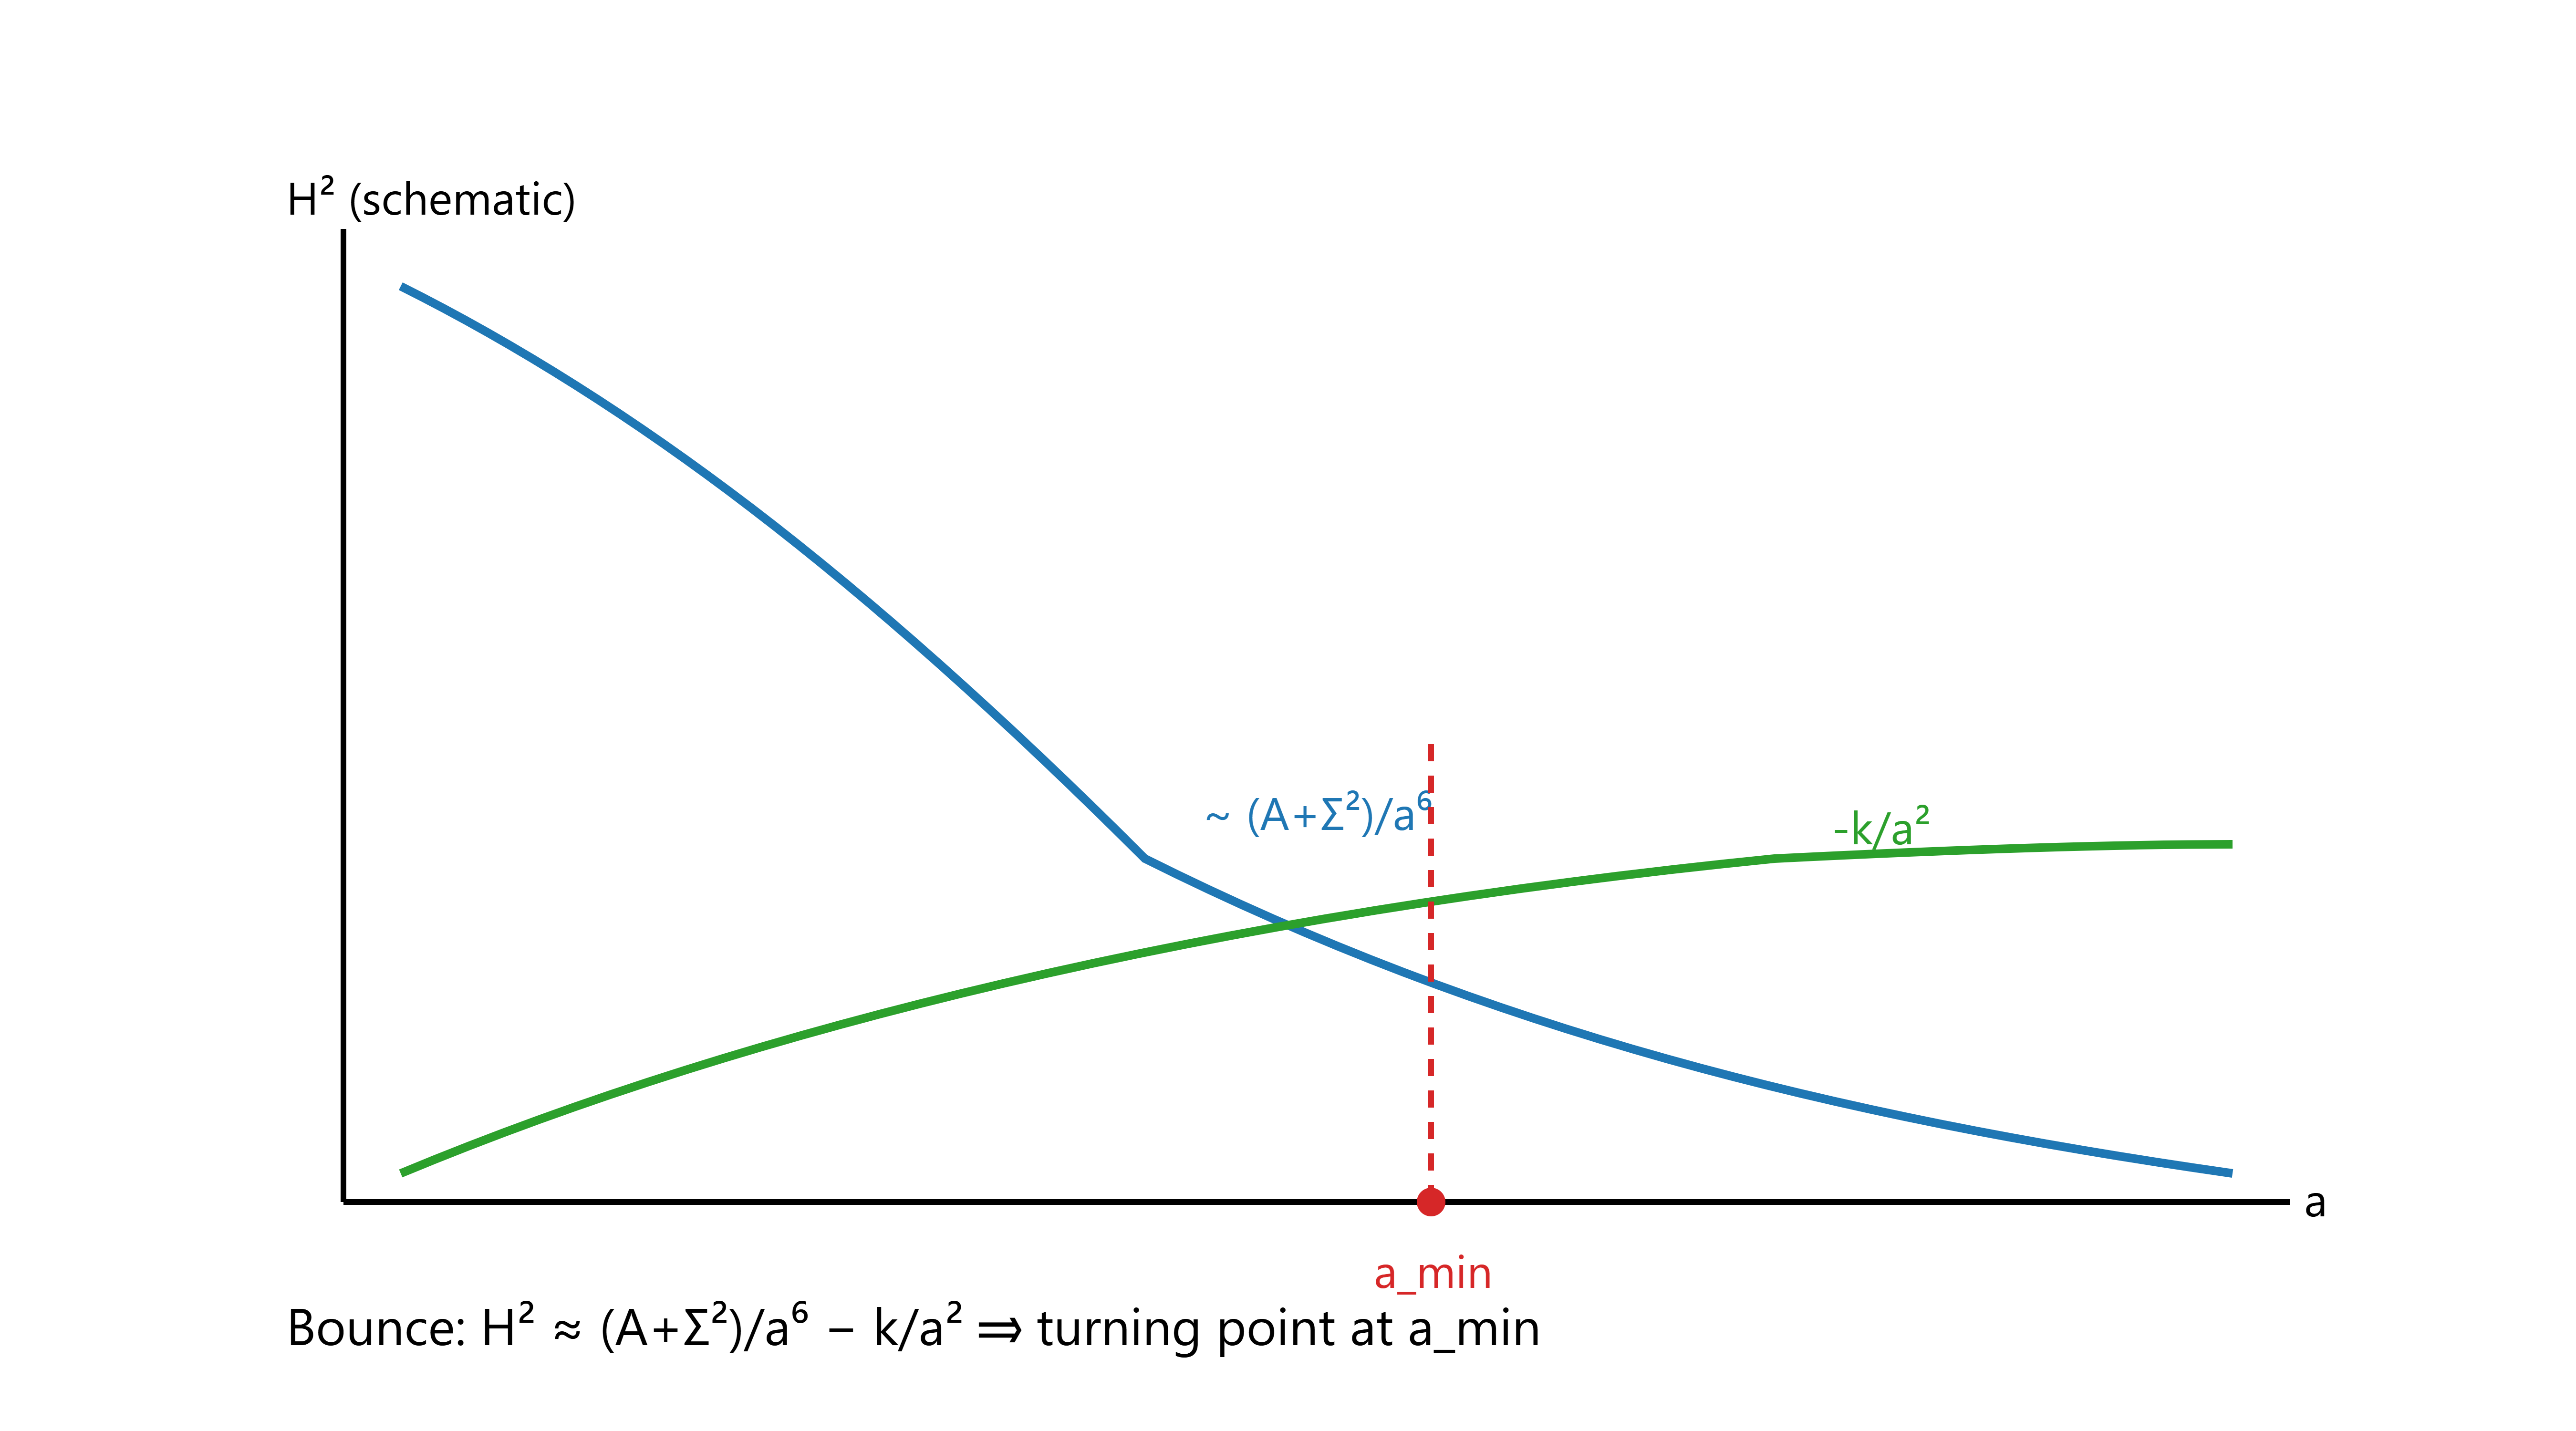
\includegraphics[width=\linewidth]{S4_bounce_schematic.png}
    \caption{Bounce schematic}
    \label{fig:bounce-schematic}
  \end{subfigure}\hfill
  \begin{subfigure}[b]{0.48\linewidth}
    \centering
  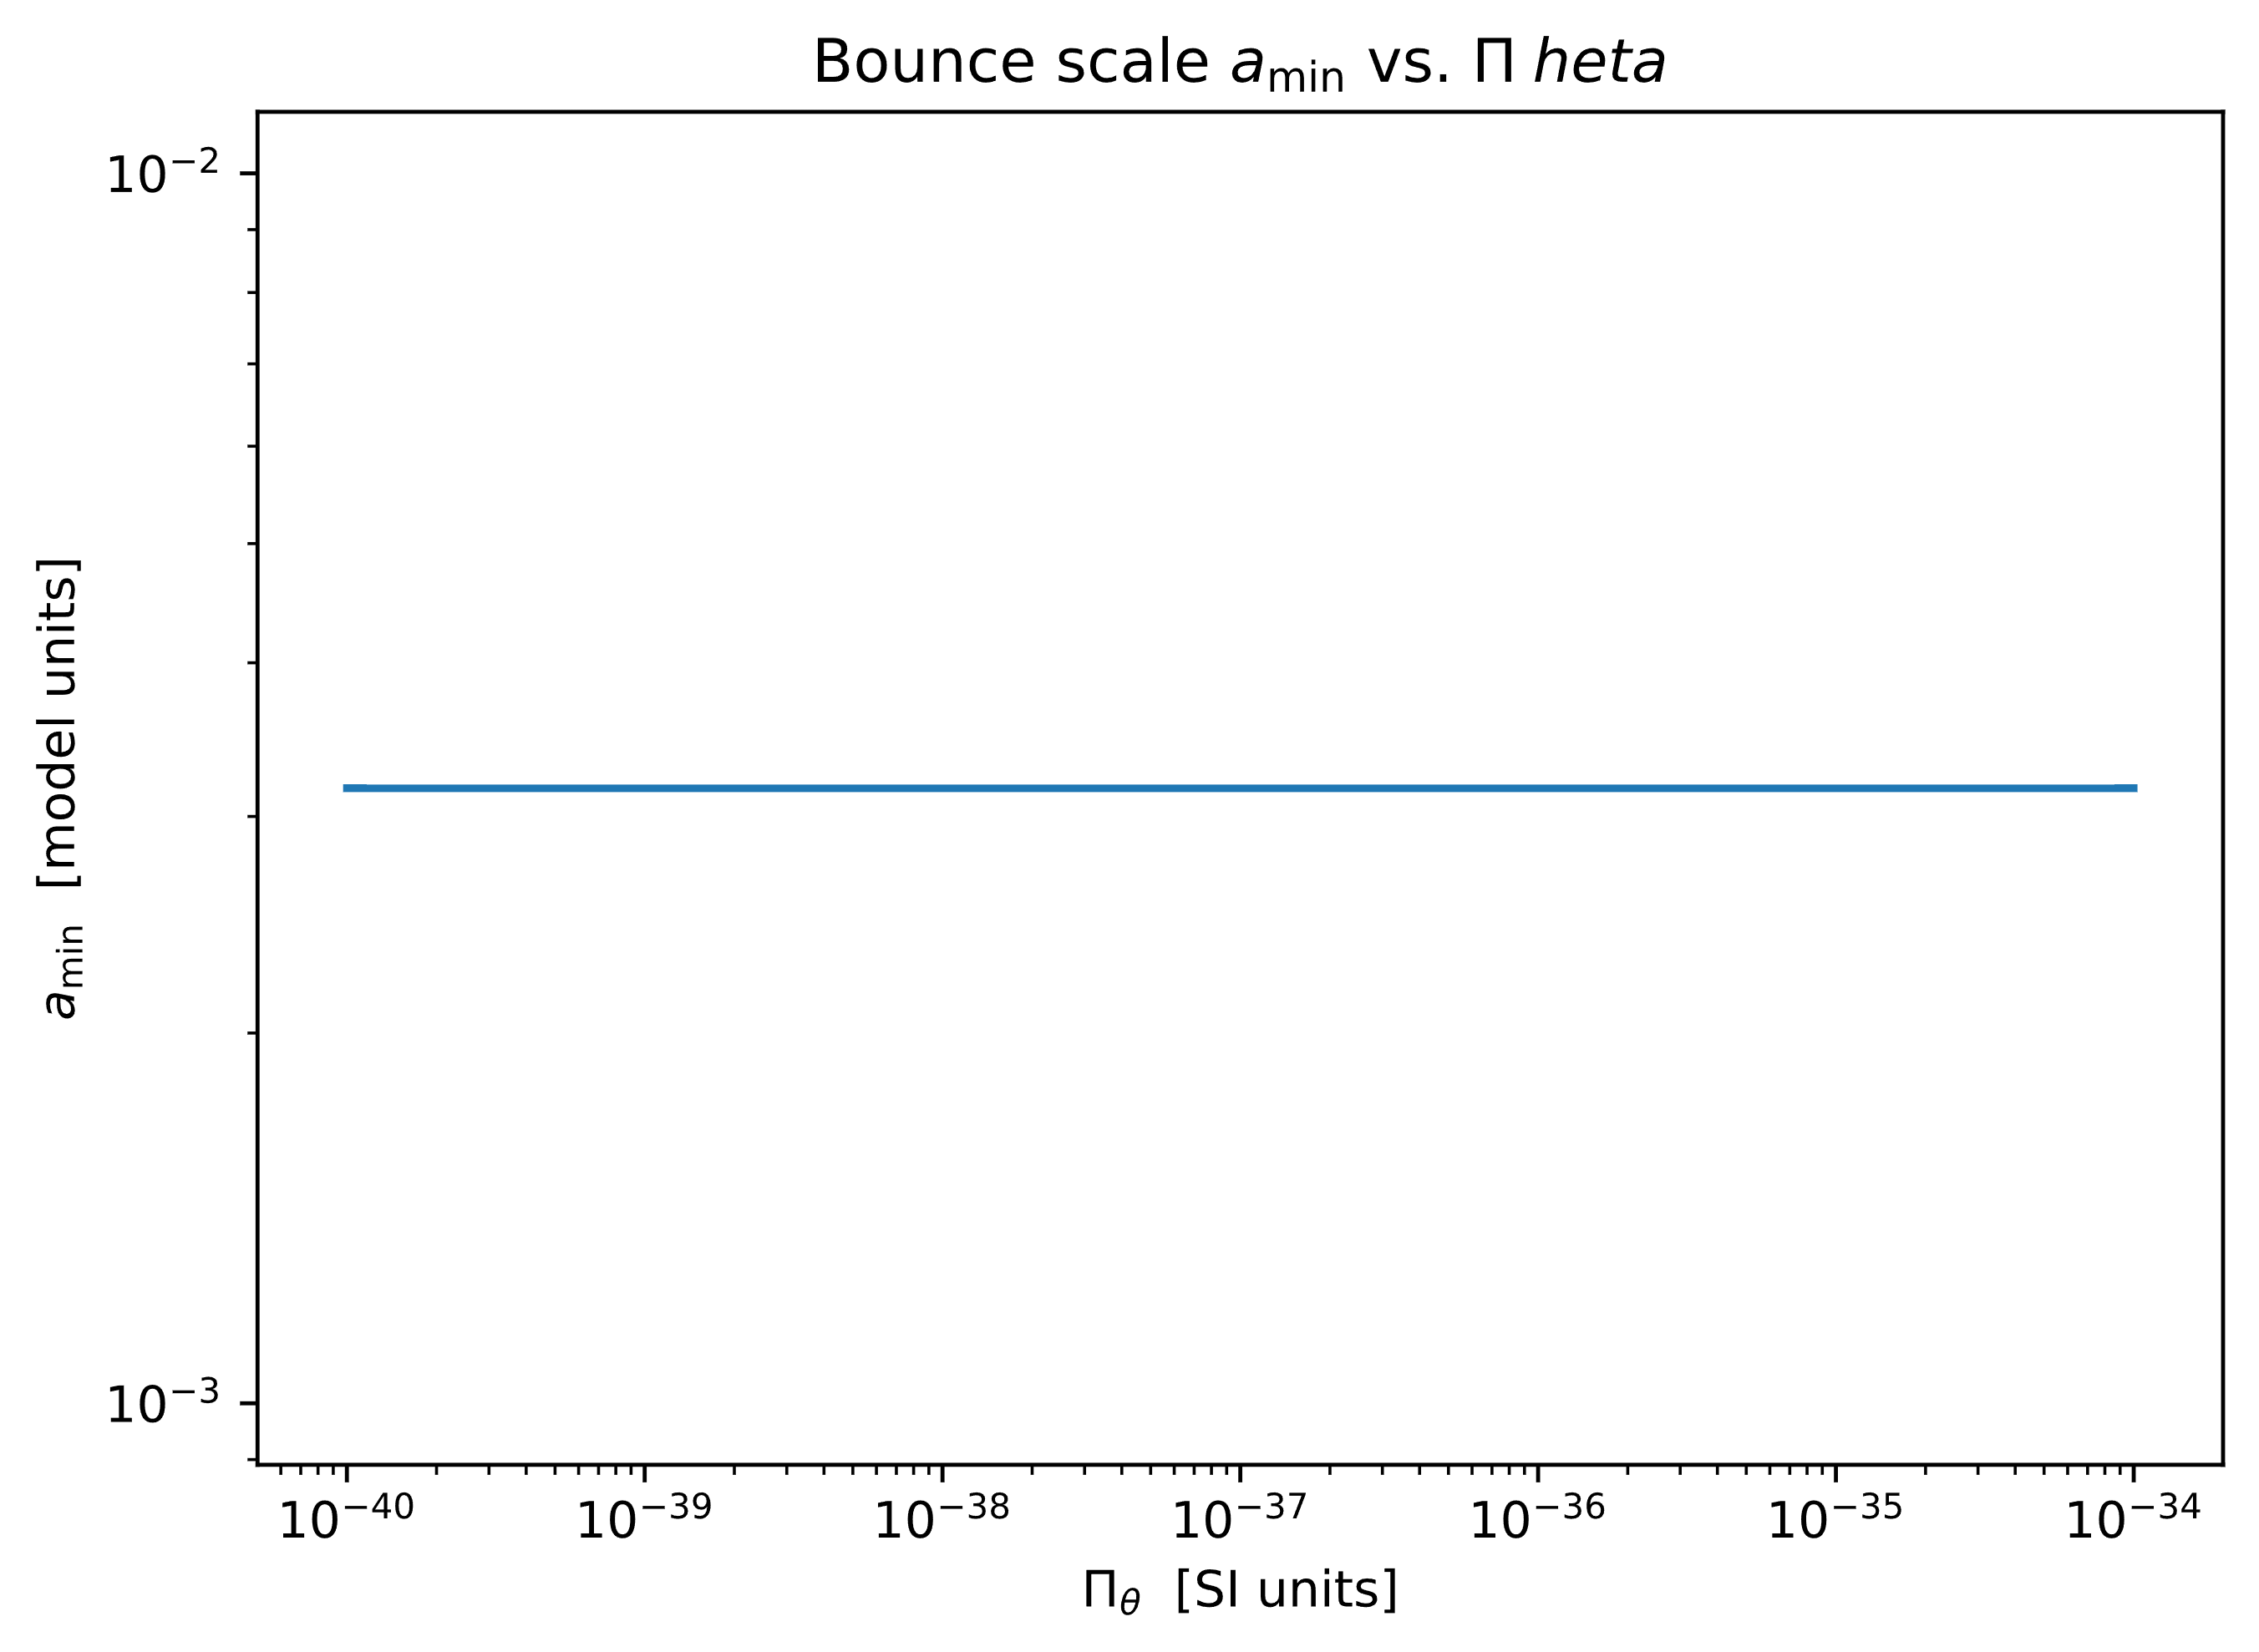
\includegraphics[width=\linewidth]{exp4_bounce_scan.png}
    \caption{Bounce scan (simulation)}
    \label{fig:bounce-scan}
  \end{subfigure}
  \caption{Classical bounce: schematic and simulation turning point.}
  \label{fig:bounce}
\end{figure}

\csvnote{../paper/data/exp4_bounce_scan.csv}

\subsection{Wheeler--DeWitt (quantum) wall at \texorpdfstring{$a=0$}{a=0}}\label{sec:wdw}
Separation $\Psi(a,\theta)=\chi(a)e^{i\ell\theta}$ gives
\begin{equation}
 \left[-\partial_a^2 + U(a) + \frac{\ell^2\hbar^2}{2 I_0 a^2}\right]\chi(a)=0,
\end{equation}
so the $+C/a^2$ term (with $C\propto \ell^2\hbar^2/I_0$) is a repulsive inverse-square barrier. Appropriate boundary conditions (or limit-point behavior for large enough $C$) yield a self-adjoint Hamiltonian and unitary evolution.

\section{Simulation Playbook (Minimal Viable Demos)}\label{sec:simulation-playbook}
Grid-based split-step evolution of a Gaussian packet on $(x,y)$ with a discrete $\theta$ ladder demonstrates cross-Hall drift and $\theta$--AB phases. Key readouts: centroid drift $\langle y(t)\rangle$, interferometric phase vs. $\oint A_\theta d\theta$, and Fourier spectra showing $\Delta E\approx \hbar^2/(2I)$.

\section*{Simulation Assumptions \& Limitations}
\begin{tcolorbox}
\textbf{Numerics.} Split\textendash step propagation on $(x,y)$; internal rotor treated via fixed Fourier index $\ell$.
Time step satisfies the spatial CFL bound. Grids: $N_x{=}N_y$ (reported per run).

\textbf{Physics scope.} No interparticle interactions; no decoherence or technical noise; classical $A_\theta(t,y)$ profiles; no back-reaction on $\theta$ dynamics.

\textbf{Boundaries.} Periodic in $x,y$ for FFT (packet remains well inside domain). 

\textbf{Validation.} Code reproduces free-packet propagation and agrees with analytic $T^2$ drift scaling for linear $A_\theta$ gradients within numeric error.

\textbf{Implication.} Sim results demonstrate \emph{internal consistency} and \emph{detectability estimates}; they are not substitutes for measured data in the proposed setups.
\end{tcolorbox}

\section{Reserved --- Open for Future Extensions}\label{sec:reserved-5}
This placeholder reserves numbering continuity for a future section (e.g., condensed-matter analogs or extended data).

\section{Unified Force --- Fixed-Core (St\"uckelberg) Edition}\label{sec:unified-force}
I promote the fiber angle to a 4D field $\Theta(x)$ and the fiber connection to a 4D gauge field $A_{\theta\mu}(x)$. A St\"uckelberg mass $m_\theta = g_\theta f_\theta$ gives a single Yukawa range $\lambda_\theta = 1/m_\theta$.

\subsection{From \texorpdfstring{$Q$}{Q} to 4D: fields and covariant derivatives}
Pullback of the connection on $Q=\mathbb R^{3,1}\times S^1$: $\Theta(x)$ and $A_{\theta\mu}(x)$. $D_\mu\Theta = \partial_\mu\Theta - g_\theta A_{\theta\mu}$; for matter, $D_\mu\psi = (\cdots + i g_\theta Q_\theta A_{\theta\mu})\psi$.

\subsection{Lagrangian core and mass}
\begin{equation}
\mathcal{L} \supset -\tfrac14 F^{(\theta)}_{\mu\nu} F_{(\theta)}^{\mu\nu} + \tfrac{f_\theta^2}{2}\,(\partial_\mu \Theta - g_\theta A_{\theta\mu})^2 - \tfrac{\varepsilon_Y}{2}\,F^{(\theta)}_{\mu\nu} B^{\mu\nu} - \tfrac{\varepsilon_2}{2}\,F^{(\theta)}_{\mu\nu} W^{3\,\mu\nu} + g_\theta A_{\theta\mu} J_\theta^\mu + \mathcal{L}_{\rm SM}.
\end{equation}
Unitary gauge ($\Theta=0$): $m_\theta=g_\theta f_\theta$, hence $\lambda_\theta=1/m_\theta$.

\subsection{Distance-law modifications with a shared range \texorpdfstring{$\lambda_\theta$}{lambda-theta}}
Massive spin-1 exchange between static sources (Born approximation):
\[
  V(r) = \mathrm{sgn}(Q_a Q_b)\, \frac{|g_a g_b|}{4\pi}\, \frac{e^{-m_\theta r}}{r}.
\]

Gravity (fifth force):
\[
  V_G(r) = -\frac{G m_1 m_2}{r}\Bigl[1 + \alpha_G e^{-r/\lambda_\theta}\Bigr],
  \quad \alpha_G = \frac{g_\theta^2\,\beta^2}{4\pi G}\ \text{if } Q_\theta=\beta m.
\]

QED (kinetic mixing):
\[
  V_{\rm EM}(r) = \frac{\alpha Q_1 Q_2}{r}\; +\; \varepsilon^2\,\alpha\, \frac{Q_1 Q_2}{r}\, e^{-r/\lambda_\theta}.
\]

See also the rotor ladder shift in Fig.~\ref{fig:ug-rotor} for an intuitive picture of holonomy.

\begin{idea}
                  	\textbf{Ladder and shift.} Energy levels are like notes on a scale, with spacing set by $I$. Holonomy $\phi_\theta$ slides the whole ladder:
$E_\ell=\tfrac{\hbar^2}{2I}\bigl(\ell-\phi_\theta/2\pi\bigr)^2$. (Skater picture: pull arms in $\Rightarrow$ smaller $I$ and wider spacing.)
\end{idea}

\begin{figure}[htbp]
  \centering
  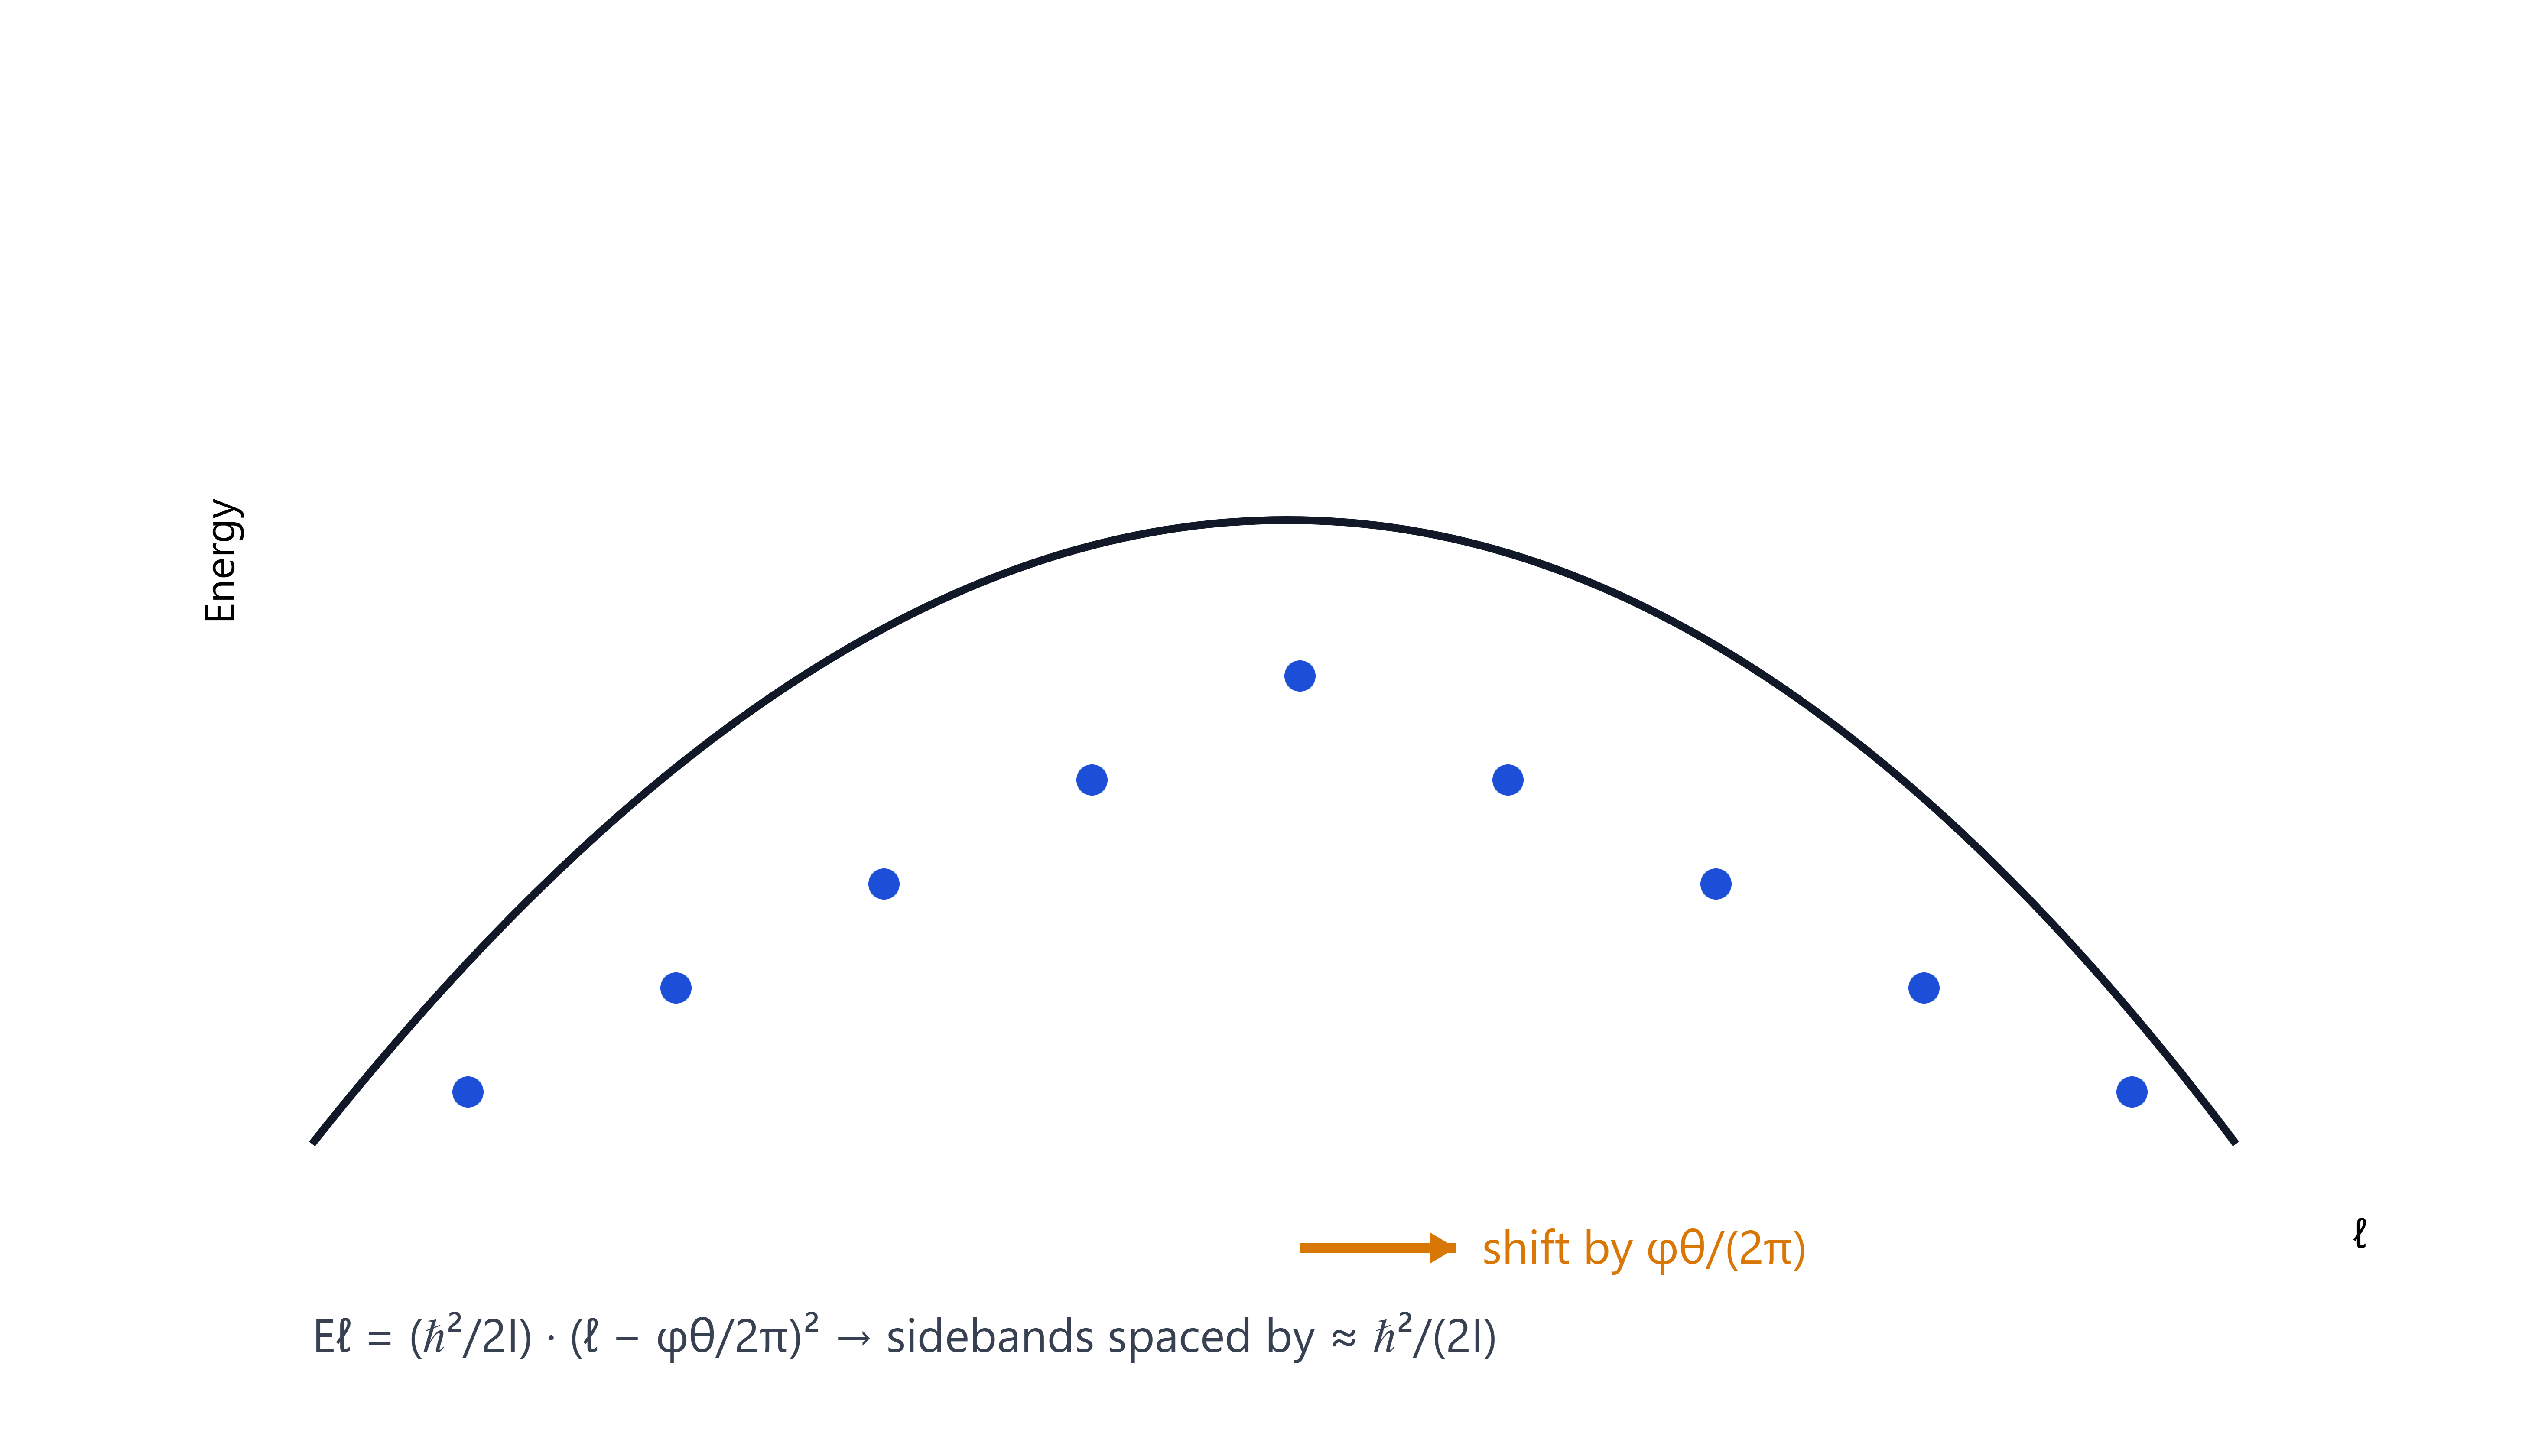
\includegraphics[width=\linewidth]{UG_S3_rotor_ladder.png}
  \caption{Rotor ladder with holonomy shift: the minimum moves by $\phi_\theta/2\pi$.}
  \label{fig:ug-rotor}
\end{figure}

\begin{figure}[htbp]
  \centering
  \begin{subfigure}[b]{0.48\linewidth}
    \centering
    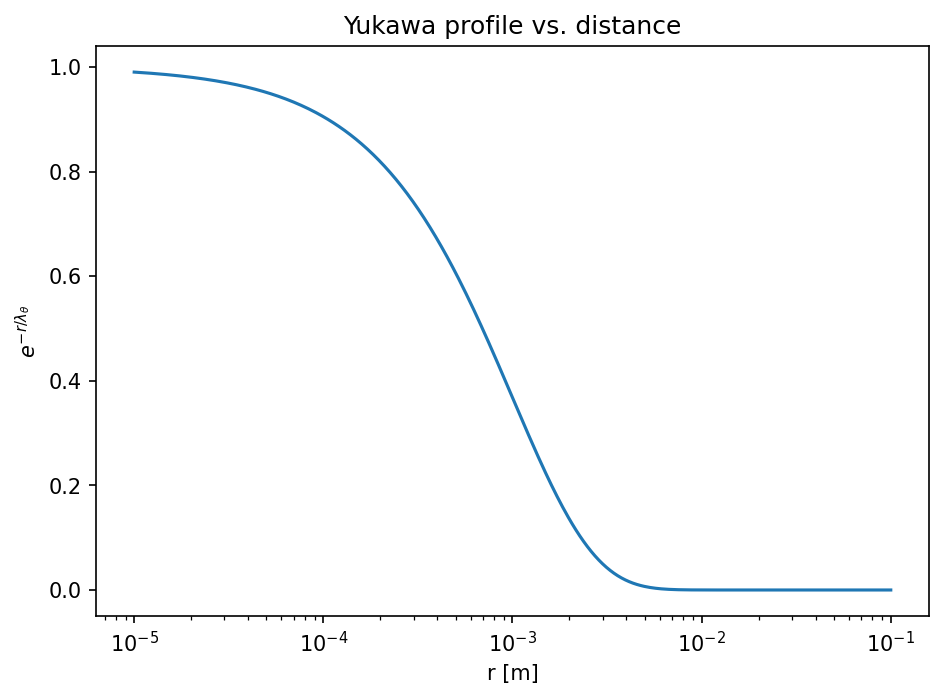
\includegraphics[width=\linewidth]{exp5_yukawa_profile.png}
    \caption{Yukawa profile $V(r)$}
    \label{fig:yukawa-profile}
  \end{subfigure}\hfill
  \begin{subfigure}[b]{0.48\linewidth}
    \centering
    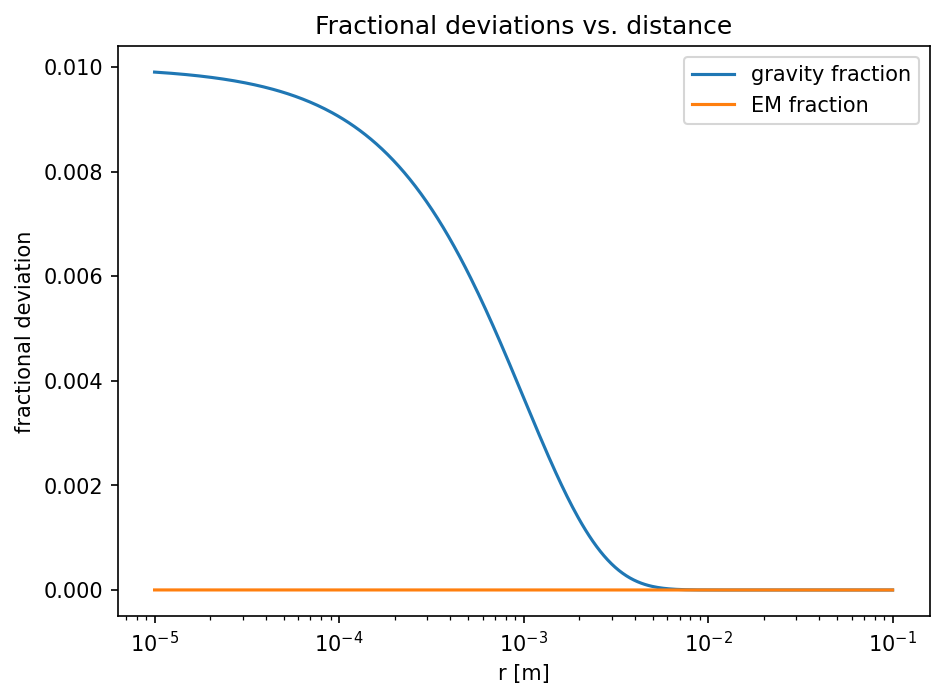
\includegraphics[width=\linewidth]{exp5_fractional_deviation.png}
    \caption{Fractional deviation vs distance}
    \label{fig:yukawa-deviation}
  \end{subfigure}
  \caption{Shared-range $\lambda_\theta$ across sectors.}
  \label{fig:yukawa}
\end{figure}

\section{Notation \& Symbols (quick lookup)}\label{sec:notation}
\noindent This page is a compact symbol list. For one-paragraph definitions and analogies, see Appendix~\ref{sec:appendix-b}.
\begin{itemize}
  \item Base coordinates: $X^\mu$ (or $X\in\mathbb R^3$ in NR limit); fiber: $\theta\in S^1$.
  \item Potentials: $A_\mu, A_\theta$; scalar potential $\phi\equiv A_0$.
  \item Curvatures: $G_{\mu\nu}=\partial_\mu A_\nu-\partial_\nu A_\mu$, $G_{\mu\theta}=\partial_\mu A_\theta-\partial_\theta A_\mu$.
  \item Charges: $q_X$ (base $U(1)$), $q_\theta$ (fiber $U(1)$). Inertia: $I$.
  \item Holonomy: $\phi_\theta\equiv( q_\theta/\hbar)\oint A_\theta\,d\theta\ (\bmod\ 2\pi)$.
  \item FRW: $a,k,\Sigma^2$; mode index $\ell$; conserved $\Pi_\theta$.
\end{itemize}

\section*{Glossary \& Notation (Quick Reference)}
For a compact symbol list, see Notation \& Symbols on \cref{sec:notation}. This appendix expands key terms with one-paragraph definitions and analogies.
\begin{description}
  \item[$Q$] Configuration space: $Q=\mathbb{R}^{3,1}\times S^1$ with coordinates $q^a=(X^\mu,\theta)$; $\theta$ is $2\pi$-periodic.
  \item[$\theta$] Compact internal angle (the ``dial''). Motion $\dot\theta$ is along the fiber, not in real space.
  \item[Compact $S^1$] The compact dimension; an angle with period $2\pi$.
    \begin{itemize}
      \item \textbf{Analogy:} garden hose looks 1D from afar, but has a circular cross-section up close.
    \end{itemize}
  \item[$A$ (connection)] Gauge connection 1-form on $Q$: $A=A_a\,dq^a= A_\mu\,dX^\mu + A_\theta\,d\theta$.
    \begin{itemize}
      \item \textbf{Analogy:} navigation tool that keeps phase transport consistent.
    \end{itemize}
  \item[$A_\theta$] Internal gauge potential along $\theta$; units $[A_\theta]=\hbar/q_\theta$ so $q_\theta A_\theta$ carries momentum.
  \item[$A_\mu,\ \phi,\ \mathbf B$] Spatial-temporal potential $A_\mu=(\phi,\mathbf A)$ with $\phi\equiv A_0$ and $\mathbf B=\nabla\times \mathbf A$.
  \item[$G=dA$] Curvature (field strength) 2-form with components $G_{ab}=\partial_aA_b-\partial_bA_a$; measures loop holonomy.
  \item[$G_{\mu\theta}$] Mixed curvature: $G_{\mu\theta}=\partial_\mu A_\theta-\partial_\theta A_\mu$; in gauge $\partial_\theta A_\mu=0$, $G_{i\theta}=\partial_i A_\theta$.
    \begin{itemize}
      \item \textbf{Analogy:} meshed gears; motion in one axis drives the other.
    \end{itemize}
  \item[$\phi_\theta$] Effective flux: $\phi_\theta \equiv \tfrac{q_\theta}{\hbar}\oint A_\theta\,d\theta$; physics is $\bmod\,2\pi$.
  \item[Holonomy] Loop-induced phase; for the fiber it is $\phi_\theta$ above. Only $\phi_\theta\ (\mathrm{mod}\ 2\pi)$ is observable.
    \begin{itemize}
      \item \textbf{Analogy:} compass twist after hiking a closed loop.
    \end{itemize}
  \item[Cross-Hall drift] Sideways drift $\propto\partial_i A_\theta$ (i.e., $G_{i\theta}$) when the fiber potential varies across space; appears even for $\mathbf E=\mathbf B=0$.
  \item[Rotor (internal)] $\theta$-motion behaves like a rotor with levels
    $\displaystyle E_\ell=\frac{\hbar^2}{2I}\Big(\ell-\frac{\phi_\theta}{2\pi}\Big)^2$, spacing $\Delta E\approx \hbar^2/(2I)$.
  \item[$I$] Rotor (phase) inertia controlling sideband spacing $\Delta E\approx \hbar^2/(2I)$; NR map $I=m\kappa^2$.
    \begin{itemize}
      \item \textbf{Analogy:} heavier flywheel $\Rightarrow$ closer level spacing.
    \end{itemize}
  \item[$m_\theta,\ \lambda_\theta$] St\"uckelberg mediator mass $m_\theta=g_\theta f_\theta$; Yukawa range $\lambda_\theta\equiv 1/m_\theta$.
  \item[$\Sigma^2$] Positive shear-like contribution $\propto a^{-6}$ in $H^2$ (early-time).
  \item[$q_X,\ q_\theta$] Charges coupling to $A_\mu$ and $A_\theta$; minimal coupling $\mathbf p\to\mathbf p-q_X\mathbf A$, $p_\theta\to p_\theta-q_\theta A_\theta$.
  \item[Large gauge] Large $\theta$-loop: $\oint A_\theta d\theta\to \oint A_\theta d\theta+2\pi\,\hbar/q_\theta$; only $\phi_\theta$ modulo $2\pi$ is physical.
  \item[Einbein $e(\tau)$] Worldline multiplier ensuring reparametrization invariance; varying it imposes the mass-shell constraint; identifies $I=m\kappa^2$.
\end{description}

\section{Related Work \& Originality}\label{sec:related-work}
I keep detailed comparisons (e.g., Kaluza--Klein, dark photon) concise here and emphasize what is original: a shared-range $\lambda_\theta$ cross-sector test, $\theta$--AB at null EM, curvature-assisted bounce with WDW barrier, and the compact-fiber vacuum lever.

\section*{Comparative Analysis with Existing Frameworks}

\begin{table}[h]
\centering
\caption{Contrast of X\textendash $\theta$ with Kaluza\textendash Klein (KK) and String Theory (ST).}
\begin{tabular}{@{}p{3.2cm}p{3.7cm}p{3.7cm}p{3.7cm}@{}}
\toprule
 & \textbf{X\textendash $\theta$} & \textbf{Kaluza\textendash Klein} & \textbf{String Theory} \\
\midrule
Extra structure & 1D \emph{fiber} angle $\theta$ over spacetime; lab\textendash programmable holonomy & Extra spatial dimensions compactified (fixed geometry) & 10D/11D with compactification; rich moduli \\
Gauge origin & $U(1)_\theta$ with St\"uckelberg mass $m_\theta$ & Gauge from higher\textendash dimensional metric components & Gauge from worldsheet/brane symmetries \\
Lab falsifiability & Direct: $\theta$\textendash AB, $T^2$ drift, rotor sidebands & Indirect: KK masses typically far above lab scales & Mostly high scale; low\textendash energy windows are model dependent \\
Single\textendash range test & Yes: one $\lambda_\theta$ across gravity/EM/weak & No single universal short range & Not generally a single range \\
Cosmo hook & Stiff $a^{-6}$ + WDW barrier, bounce scale tied to lab $I$ & Exotic matter from geometry; no simple lab knob & Early\textendash universe from string cosmology; many scenarios \\
EP hygiene & $Q_\theta\propto m$ or $B\!\textendash\!L$ $\Rightarrow$ leading EP\textendash safe & Composition dependence model\textendash dependent & Model\textendash dependent \\
\bottomrule
\end{tabular}
\end{table}

\section{Vacuum Energy in X--\texorpdfstring{$\theta$}{theta}: From Knife-Edge to Relaxation}\label{sec:vacuum-energy}
Sketch of how the compact fiber can modify vacuum contributions; a full treatment is reserved for future work.

\section*{Data \& Code Availability}
All figure data are provided as CSV in \texttt{../paper/data/} and raster/vector figures in \texttt{../paper/figs/}.  
Repository (simulation notebooks and build scripts): 
\href{https://github.com/divyang4481/X-theta-framework}{github.com/divyang4481/X-theta-framework}.

\noindent Example links used in this paper: 
\texttt{../paper/data/exp1\_theta\_ab\_fringe.csv}, 
\texttt{../paper/data/exp2\_drift\_T2.csv}, 
\texttt{../paper/data/exp3\_rotor\_levels.csv}, 
\texttt{../paper/data/exp4\_bounce\_scan.csv}, 
\texttt{../paper/data/exp5\_yukawa\_profiles.csv}.

\bigskip
\noindent Correspondence: \texttt{22f1000411@ds.study.iitm.ac.in}; \texttt{divyang4481@gmail.com}

\noindent License: CC BY-SA 4.0

\appendix
\section*{Appendix A --- Cross-Hall Drift Coefficient (paraxial beam)}\label{sec:appendix-a}
\addcontentsline{toc}{section}{Appendix A --- Cross-Hall Drift Coefficient}
Assuming a paraxial Gaussian $\psi(X,\theta,t)=\Phi(X,t)\,\chi(\theta,t)$ and slowly varying $A_\theta(X)$ across waist $w_0$, treating $G_{i\theta}=\partial_iA_\theta$ as uniform and linearizing the moments gives
\begin{equation}
 \frac{d^2}{dt^2}\langle X_i\rangle = \frac{q_\theta}{m}\,(\partial_iA_\theta)\,\langle\dot\theta\rangle + \mathcal O(w_0^{-2},\partial_i^2A_\theta),
\end{equation}
so a square gate of duration $T$ yields $\Delta X_i = \alpha\,\frac{q_\theta}{m}\,(\partial_iA_\theta)\,\frac{T^2}{2}\,\langle\dot\theta\rangle$ with $\alpha\approx 1$ (top-hat) and $\alpha<1$ (Gaussian).

\section*{Appendix B --- Glossary}\label{sec:appendix-b}
\addcontentsline{toc}{section}{Appendix B --- Glossary}
\begin{description}
  \item[Holonomy] Loop-induced phase from parallel transport around the fiber:
  \[
    \Delta\varphi_\theta=\frac{q_\theta}{\hbar}\oint A_\theta\,d\theta \equiv \phi_\theta\ (\mathrm{mod}\ 2\pi).
  \]
  \begin{itemize}
    \item \textbf{Analogy:} hiking a loop around a hill and finding your compass rotated when you return.
    \item \textbf{Where:} \cref{sec:theta-ab}.
  \end{itemize}

  \item[Mixed curvature $G_{\mu\theta}$] Coupling between base and fiber:
  \[
    G_{\mu\theta}=\partial_\mu A_\theta-\partial_\theta A_\mu,\quad \text{with}\; \partial_\theta A_\mu=0\Rightarrow G_{i\theta}=\partial_i A_\theta.
  \]
  \begin{itemize}
    \item \textbf{Analogy:} a gear train linking forward motion and an internal wheel.
    \item \textbf{Where:} \cref{sec:cross-hall}.
  \end{itemize}

  \item[Minisuperspace] Truncated configuration space for homogeneous modes (e.g., $(a,\theta)$ in FRW).
  \begin{itemize}
    \item \textbf{Analogy:} a city map showing only two main avenues.
    \item \textbf{Where:} \cref{sec:cosmology}.
  \end{itemize}

  \item[Inverse-square barrier] Repulsive $+C/a^2$ term in the Wheeler--DeWitt (WDW) equation, with threshold for essential self-adjointness at $\gamma\ge 3/4$ for $-\chi''+\tfrac{\gamma}{a^2}\chi$.
  Here $C\propto \ell^2\hbar^2/I_0$.
  \begin{itemize}
    \item \textbf{Where:} \cref{sec:wdw}.
  \end{itemize}

  \item[Phase stiffness / inertia $I$] Sets rotor sideband spacing $\Delta E\approx \hbar^2/(2I)$. NR map: $I=m\kappa^2$.
  \begin{itemize}
    \item \textbf{Analogy:} a heavier flywheel has more closely spaced levels.
    \item \textbf{Where:} \cref{sec:sidebands}.
  \end{itemize}

  \item[Einbein $e(\tau)$] Worldline multiplier enforcing reparametrization invariance; varying it imposes the mass-shell constraint. In the relativistic map one finds $I=m\kappa^2$.
  \begin{itemize}
    \item \textbf{Where:} \cref{sec:relativistic-worldline}.
  \end{itemize}

  \item[Gauge connection $A$] One-form on $Q$ that tracks phase transport:
  $A= A_\mu\,dX^\mu + A_\theta\,d\theta$, with curvature $G=dA$.
  \begin{itemize}
    \item \textbf{Analogy:} navigating a boat with changing currents.
    \item \textbf{Where:} \cref{sec:gauge-invariance}.
  \end{itemize}

  \item[Compact dimension $S^1$] Fiber coordinate $\theta$ is an angle with period $2\pi$.
  \begin{itemize}
    \item \textbf{Analogy:} a garden hose looks 1D from far away but has a circular cross-section up close.
    \item \textbf{Where:} \cref{sec:framework}.
  \end{itemize}

  \item[Flux quanta and large gauge] The $U(1)_\theta$ flux quantum is $\Phi_{\theta,0}=2\pi\hbar/q_\theta$; large $\theta$-loops shift $\oint A_\theta d\theta$ by $2\pi\hbar/q_\theta$, so only $\phi_\theta$ modulo $2\pi$ is physical.
  \begin{itemize}
    \item \textbf{Where:} \cref{sec:gauge-invariance}.
  \end{itemize}

  \item[Rotor (internal) and sidebands] With $\psi\sim e^{i\ell\theta}$, levels are
  \[
    E_\ell=\frac{\hbar^2}{2I}\Big(\ell-\frac{\phi_\theta}{2\pi}\Big)^2,\quad \ell\in\mathbb Z,
  \]
  giving near-harmonic sidebands spaced by $\Delta E\approx \hbar^2/(2I)$.
  \begin{itemize}
    \item \textbf{Where:} \cref{sec:sidebands}.
  \end{itemize}

  \item[Stueckelberg mass $m_\theta$ and Yukawa range $\lambda_\theta$] In 4D, $m_\theta=g_\theta f_\theta$ and $\lambda_\theta\equiv 1/m_\theta$. The same $\lambda_\theta$ controls short-range fingerprints across gravity/QED/weak sectors.
  \begin{itemize}
    \item \textbf{Where:} \cref{sec:unified-force}.
  \end{itemize}

  \item[Kinetic mixing $\varepsilon$] $U(1)$--$U(1)$ mixing induces a small Yukawa bump in Coulomb's law.
  \begin{itemize}
    \item \textbf{Analogy:} two pendulums tied by a weak spring.
    \item \textbf{Where:} \cref{sec:unified-force}.
  \end{itemize}

  \item[Cross-Hall drift] Transverse drift proportional to $\partial_i A_\theta$ when the fiber potential varies across space; see also Appendix~\ref{sec:appendix-a} for a paraxial coefficient.
  \begin{itemize}
    \item \textbf{Where:} \cref{sec:cross-hall}.
  \end{itemize}

  \item[Charges $q_X,\ q_\theta$] Minimal coupling rules: $\mathbf p\to\mathbf p-q_X\mathbf A$ and $p_\theta\to p_\theta-q_\theta A_\theta$.
  \begin{itemize}
    \item \textbf{Where:} \cref{sec:framework}.
  \end{itemize}
\end{description}


% Bibliography
\clearpage
% Include all references even if not cited
\nocite{*}
\bibliographystyle{unsrt}
\bibliography{refs}

\end{document}
